% Generated by report/build_report.py --ieee. Do not edit by hand: change the script and rebuild.
\documentclass[conference]{IEEEtran}
\usepackage{amsmath,amssymb,graphicx,textcomp,booktabs,array}
\renewcommand{\ttdefault}{cmtt}
\newlength{\tabw}
\makeatletter
\newcommand{\linebreakand}{\end{@IEEEauthorhalign}\hfill\mbox{}\par\mbox{}\hfill\begin{@IEEEauthorhalign}}
\makeatother
\setlength{\emergencystretch}{2em}
\begin{document}
\title{Maze Runner: Comparing Uninformed and Heuristic Search in Grid Mazes\\[2pt]{\Large\itshape When does the A* heuristic stop helping?}}
\author{\IEEEauthorblockN{Aaliyan Muhammad}
\IEEEauthorblockA{251357591 \\ CS3346A, Group 26 \\ Dept. of Computer Science \\ Western University, London, Canada}
\and
\IEEEauthorblockN{Austin Brown}
\IEEEauthorblockA{251446658 \\ CS3346A, Group 26 \\ Dept. of Computer Science \\ Western University, London, Canada}
\and
\IEEEauthorblockN{Aryan Farhang}
\IEEEauthorblockA{251311878 \\ CS3346A, Group 26 \\ Dept. of Computer Science \\ Western University, London, Canada}
\linebreakand
\IEEEauthorblockN{Ki il Eum}
\IEEEauthorblockA{251181143 \\ CS3346A, Group 26 \\ Dept. of Computer Science \\ Western University, London, Canada}
\and
\IEEEauthorblockN{Yicheng Luo}
\IEEEauthorblockA{251248739 \\ CS3346A, Group 26 \\ Dept. of Computer Science \\ Western University, London, Canada}}
\maketitle
\begin{abstract}
Breadth-first search (BFS) and A* both return shortest paths in a grid maze, but A* is supposed to get there with less work because a heuristic points it toward the goal. We test when that is true. We built a reproducible Python experiment that generates seeded mazes, runs BFS, uniform cost search (UCS) and A* with the Manhattan distance heuristic through one shared graph-search loop, and checks every returned path with an independent verifier. The data are synthetic: 2,650 maze instances from fixed seeds, covering perfect mazes (one route), looped mazes (extra walls removed) and weighted mazes (mud that costs 5), from 10$\times$10 to 100$\times$100 cells. All 9,350 search runs returned legal paths, and all 7,550 runs of algorithms that guarantee optimality were optimal. On perfect mazes A* expanded only 6.3\% (50$\times$50) and 3.7\% (100$\times$100) fewer nodes than BFS, far below our 30\% target. On looped mazes it saved 38.1\% and 24.4\%, so the target was met at 50$\times$50 and not met at 100$\times$100. Savings track how informed the heuristic is, measured as h(start)/C*: below 0.4 they exceeded 30\% on only 13 of 248 mazes. An exact heuristic is still not enough: on open grids A* with first-in-first-out tie-breaking saved nothing, while preferring deeper nodes saved up to 99\%. With mud, A* and UCS always agreed on cost, the advantage of A* shrank to 3.1\% at 100$\times$100, and BFS paths cost 5.9\% more than the optimum on average.
\end{abstract}
\begin{IEEEkeywords}
heuristic search, A*, breadth-first search, uniform cost search, maze generation, tie-breaking, reproducibility
\end{IEEEkeywords}

\section{Introduction}

Finding a good route through a space with obstacles is one of the oldest problems in artificial intelligence. A warehouse robot, a character in a video game and a delivery planner all solve some version of it. The textbook answer is state-space search, and the textbook comparison is between uninformed search, which knows nothing about where the goal is, and informed search, which uses a heuristic estimate of the remaining distance~\cite{ref4}. BFS is the standard uninformed method when every move costs the same. A*~\cite{ref1} is the standard informed method: it expands nodes in order of f = g + h, the cost so far plus the estimated cost to go.


It is tempting to summarize the comparison as ``A* is faster''. That summary hides the interesting part. A heuristic is only as useful as it is accurate, and in a maze the straight-line estimate can be badly wrong: the corridor that heads toward the goal may be a dead end, and the true route may wind through most of the maze. Our proposal named this as the failure case to study. This report is built around that question.


\textbf{Research questions.}

\begin{itemize}
  \item \textbf{RQ1.} How many fewer nodes does A* with Manhattan distance expand than BFS on perfect and looped mazes from 10$\times$10 to 100$\times$100 cells? In particular, does it meet the proposal's success criterion of at least 30\% fewer expansions on average for 50$\times$50 and larger, while always returning a shortest path?
  \item \textbf{RQ2.} When does the Manhattan heuristic stop helping, and what property of a maze predicts it?
  \item \textbf{RQ3.} When squares have different costs (mud costs 5), how do UCS and A* compare, and how wrong is BFS?
\end{itemize}

\textbf{Goals and contributions.} We set out to build a fair, checkable experiment rather than a demo. The project delivers:

\begin{itemize}
  \item a seeded maze generator for perfect, looped and weighted mazes, in which a seed always rebuilds the same maze;
  \item one graph-search loop shared by BFS, UCS, A* and greedy best-first search, so that all algorithms use the same successor function, neighbour order, duplicate rule and counters;
  \item an independent path verifier applied to every run, 1056 automated tests, and an exact reproduction of the expansion counts of the Week 3 lecture example;
  \item a held-out evaluation: all design choices were made on development seeds, the code was frozen with a git tag, and the final seeds were run once;
  \item an analysis that explains the results with a single measurable quantity, the heuristic informedness h(start)/C*, and that separates two different ways in which the heuristic stops helping.
\end{itemize}

\textbf{Structure of the report.} Section II reviews the algorithms, the properties of heuristics, maze generation and related work. Section III defines the problem formally and describes the implementation, the verification and the evaluation protocol. Section IV presents and interprets the results, including a failure case and the limitations. Section V concludes and lists future work. Section VI records individual contributions. Appendix A is the reproducibility record and Appendix B holds extra tables and figures. The code, results and report sources are available at \texttt{https:/\allowbreak{}/\allowbreak{}github.com/\allowbreak{}AryanFP/\allowbreak{}maze-runner}.


\section{Background and Related Work}

\subsection{Search problems and the algorithms compared}

A search problem is defined by a state space, the actions available in each state, a start state, a goal test and a step cost; a solution is a path from the start to a goal, and an optimal solution has the lowest total cost~\cite{ref4,ref13}. All the algorithms in this report are instances of one scheme, best-first graph search: keep a frontier of generated but unexpanded nodes, repeatedly remove one, and add its successors. They differ only in which node the frontier releases next (Table~\ref{tab:algos}).

\begin{table*}[!t]
\centering
\footnotesize
\setlength{\tabw}{\dimexpr \textwidth-10\tabcolsep\relax}
\caption{The four algorithms as frontier policies of one graph-search loop. b is the branching factor, d the depth of the shallowest goal, C* the optimal solution cost, V and E the numbers of states and edges.}
\label{tab:algos}
\begin{tabular}{>{\raggedright\arraybackslash}p{\dimexpr 0.1576\tabw\relax}>{\raggedright\arraybackslash}p{\dimexpr 0.2182\tabw\relax}>{\raggedright\arraybackslash}p{\dimexpr 0.1394\tabw\relax}>{\raggedright\arraybackslash}p{\dimexpr 0.2242\tabw\relax}>{\raggedright\arraybackslash}p{\dimexpr 0.2606\tabw\relax}}
\toprule
\textbf{Algorithm} & \textbf{Frontier order} & \textbf{Complete} & \textbf{Optimal} & \textbf{Notes} \\
\midrule
BFS~\cite{ref3} & First in, first out (shallowest first) & Yes & Yes, if all steps cost the same & Time and space O(b\textasciicircum{}d) in general; O(V + E) on an explicit graph \\
UCS (Dijkstra)~\cite{ref2} & Lowest path cost g & Yes, if costs $\geq$ $\varepsilon$ \textgreater{} 0 & Yes & Expands every node with g \textless{} C* \\
Greedy best-first & Lowest estimate h & Yes on finite graphs & No & Fast when h is good; ignores the cost already paid \\
A*~\cite{ref1} & Lowest f = g + h & Yes & Yes, if h is admissible (with reopening) or consistent & Expands every node with f \textless{} C* \\
\bottomrule
\end{tabular}
\end{table*}

BFS was described for maze routing by Moore~\cite{ref3}. It finds a path with the fewest steps, which is the cheapest path only when every step costs the same. UCS is Dijkstra's algorithm~\cite{ref2} stopped at the goal; it orders the frontier by the cost so far and is optimal for any positive step costs. Greedy best-first search orders by the heuristic alone and gives up optimality. A*, introduced by Hart, Nilsson and Raphael~\cite{ref1}, adds the two: g keeps it honest about the cost already paid and h pulls it toward the goal.


\subsection{Admissible and consistent heuristics}

Let h*(s) be the true cheapest cost from s to the goal. A heuristic is \textbf{admissible} if it never overestimates, 0 $\leq$ h(s) $\leq$ h*(s), and \textbf{consistent} if h(u) $\leq$ c(u, v) + h(v) for every edge and h(goal) = 0~\cite{ref4,ref5}. Consistency implies admissibility. With an admissible heuristic A* is optimal as long as a node can be reopened when a cheaper path to it is found; with a consistent heuristic f never decreases along a path, the first time a node is removed its g is already optimal, and no reopening is needed~\cite{ref5,ref13}. A standard way to build an admissible heuristic is to solve a \textbf{relaxed} problem with some constraints removed: the relaxed optimum can only be cheaper~\cite{ref5}. For two admissible heuristics, the larger one \textbf{dominates} and never causes more expansions with f \textless{} C*.


Two classical results frame our study. First, Dechter and Pearl~\cite{ref6} showed that A* with a consistent heuristic is optimally efficient: any algorithm that is guaranteed to be optimal using the same heuristic must expand every node with f \textless{} C*. The only freedom left is among nodes with f = C*, which is decided by tie-breaking. Second, the size of the set \{f \textless{} C*\} depends entirely on how close h is to h*. If h = h* everywhere, only nodes on optimal paths qualify; if h = 0, A* is UCS. The usefulness of A* is therefore not a property of the algorithm alone but of the heuristic in a particular environment. That is the premise of our title question.


\subsection{Maze generation}

A \textbf{perfect maze} has exactly one simple path between any two cells; as a graph it is a spanning tree of the grid. The randomized depth-first search generator, also called the recursive backtracker, carves such a tree by walking to a random unvisited neighbour and backtracking when stuck. It is known for long, winding corridors with few short dead ends~\cite{ref9}. Removing extra walls from a perfect maze creates cycles and gives a \textbf{looped} (braided) maze with more than one route between cells~\cite{ref9}. Other generators, such as randomized Prim's or Kruskal's algorithms, produce mazes with a different texture (more, shorter dead ends)~\cite{ref9}; we return to this in the limitations.


\subsection{Related work}

Grid pathfinding is a well-studied benchmark domain. Sturtevant~\cite{ref7} assembled standard benchmark sets of game maps, random obstacle maps, rooms and mazes of different corridor widths, and noted that results on one map type often do not carry over to another. Harabor and Grastien's Jump Point Search~\cite{ref8} speeds up A* on uniform-cost grids by pruning the many symmetric optimal paths that open areas create; those symmetric paths are the same f = C* ties that we measure in Section IV-C. Pohl's weighted A*~\cite{ref12} inflates the heuristic by a factor w \textgreater{} 1 to trade solution quality for speed, with cost at most w times the optimum; we use it as an ablation. More recently, learned guidance has been added on top of the same search structure: Neural A*~\cite{ref10} learns a cost map so that a differentiable A* expands fewer nodes, and Searchformer~\cite{ref11} trains a transformer on A* search traces from maze and Sokoban problems. Both were discussed in the course~\cite{ref13} and both are evaluated by counting expansions against A*, which is the metric we use.


\textbf{Why a good heuristic can still leave a lot of work.} Russell and Norvig~\cite{ref4} summarise the quality of a heuristic by its effective branching factor, and Pearl~\cite{ref5} analysed how the work done by A* grows with the error of the heuristic. Korf, Reid and Edelkamp~\cite{ref16} showed that the number of nodes expanded by iterative-deepening A* can be predicted from the distribution of heuristic values over the state space, not from the heuristic's accuracy at the start state alone. Our informedness h(start)/C* is a one-number summary of that idea, which is why we treat it as a predictor of savings and not as their cause. Helmert and R\"oger~\cite{ref14} showed that even a heuristic that is wrong by only a small constant can leave A* with exponentially many nodes to expand, because many states share f = C*. Asai and Fukunaga~\cite{ref15} studied this final plateau directly and found that the tie-breaking rule used inside it changes the number of expansions substantially; preferring nodes with smaller h, which at equal f is the same as preferring larger g, is a common default. Our open-grid result in Section IV-C, where first-in-first-out ties lose all of A*'s advantage while larger-g ties keep almost all of it, is a small and clean instance of their observation.


\textbf{Changing environments.} A robot exploring unknown terrain must replan whenever it discovers a wall. D* Lite~\cite{ref17} reuses the work of earlier searches so that replanning after a map change costs much less than searching again from scratch. Our mazes are static and fully known, so every run starts fresh; mazes that change during the search are one of the extensions in Section V.


\textbf{How this project differs.} We do not propose a new algorithm. We run a controlled study of a single factor, maze structure, and ask how it changes the value of a fixed, standard heuristic. The mazes come from one generator with one knob (the fraction of walls removed), so the heuristic's accuracy can be varied smoothly from almost useless to exact while everything else is held fixed.


\section{Methodology and Implementation}

\subsection{Problem formulation}

We use the five-part formulation from the course~\cite{ref13} (Table~\ref{tab:problem}). A maze of size n has n$\times$n cells. It is stored as an occupancy grid of (2n+1)$\times$(2n+1) squares in which every square is either a wall or open: cell (r, c) is square (2r+1, 2c+1), and the square between two neighbouring cells is open if there is a passage and a wall otherwise. Search runs on the squares. A ``50$\times$50 maze'' therefore means 50$\times$50 cells on a 101$\times$101 grid, and all path lengths in this report are in grid steps.

\begin{table}[!t]
\centering
\footnotesize
\setlength{\tabw}{\dimexpr \columnwidth-4\tabcolsep\relax}
\caption{Formal definition of the search problem.}
\label{tab:problem}
\begin{tabular}{>{\raggedright\arraybackslash}p{\dimexpr 0.1576\tabw\relax}>{\raggedright\arraybackslash}p{\dimexpr 0.8424\tabw\relax}}
\toprule
\textbf{Part} & \textbf{Definition in this project} \\
\midrule
State & The square (row, col) occupied by the agent. Nothing else changes which moves are legal or what they cost, so the position is a sufficient state. \\
Actions & Up, Right, Down, Left (always tried in this order). An action is legal if the target square is inside the grid and is not a wall. \\
Start & The top-left cell, square (1, 1). \\
Goal test & The state equals the bottom-right cell, square (2n$-$1, 2n$-$1). \\
Step cost & Unweighted mazes: 1 per move. Weighted mazes: the entry cost of the square that is entered (1 for a normal square, 5 for mud); the start is free. This is the convention of the Week 3 weighted grid example~\cite{ref13}. \\
\bottomrule
\end{tabular}
\end{table}

The correctness claims below rest on assumptions that we state explicitly, following the course checklist~\cite{ref13}: the branching factor is finite (at most 4); every step cost is positive (at least 1); the state is sufficient; repeated states are detected (graph search); and the goal is tested at the right time for each algorithm (Section III-C).


\subsection{Maze generation}

All mazes are generated by our own code from an integer seed (Fig.~\ref{fig:types}). Each maze uses its own random generator objects derived from the seed, never the global random state, so a seed always rebuilds the same maze; each maze also carries a SHA-256 fingerprint of its grid, stored in the results.

\begin{itemize}
  \item \textbf{Perfect mazes} are carved by randomized depth-first search with an explicit stack (a recursive version would exceed Python's recursion limit at 100$\times$100). The result is a spanning tree with exactly n\textsuperscript{2} $-$ 1 passages.
  \item \textbf{Looped mazes} start from the perfect maze of the same seed. A perfect maze has (n $-$ 1)\textsuperscript{2} internal walls left; we open a fraction p of them, chosen at random. The default is p = 0.1. For one seed, the opened walls at a higher p include those at a lower p, so mazes are nested across the sweep in Section IV-C.
  \item \textbf{Weighted mazes} start from a looped maze and turn a fraction m of the open squares (never the start or goal) into mud that costs 5 to enter. The default is m = 0.2. We never put mud on a perfect maze: a perfect maze has exactly one route from start to goal, so costs cannot change which path is best and BFS, UCS and A* would all return the same route. Costs only matter when there are alternative routes.
\end{itemize}

Before a maze is used, a plain flood fill confirms that the goal can be reached from the start; a failure would stop the run rather than be skipped. It never occurred.

\begin{figure*}[!t]
\centering
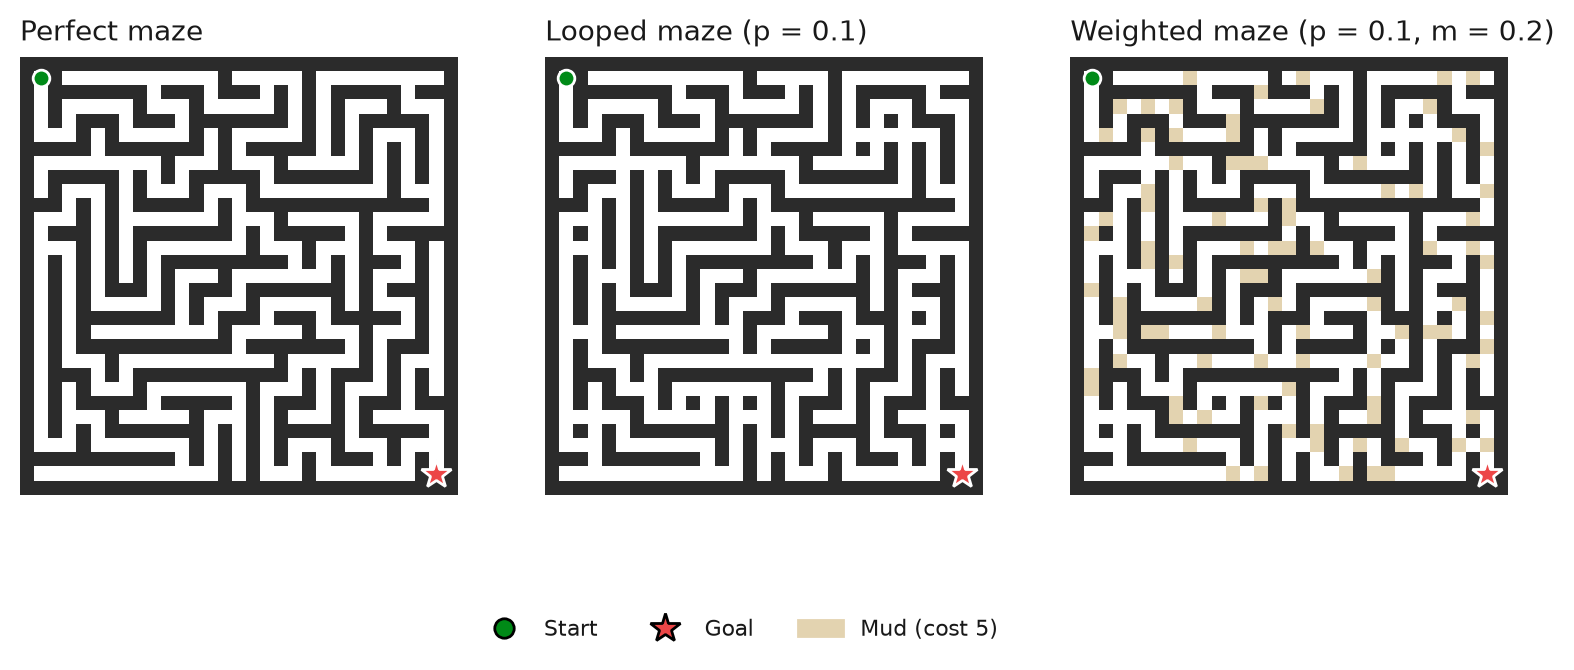
\includegraphics[width=0.97\textwidth]{figures/maze_types.png}
\caption{The three maze types for one seed (15$\times$15 cells, seed 10016, shown small for legibility). The looped maze is the perfect maze with 10\% of its remaining internal walls opened; the weighted maze adds mud on 20\% of the open squares.}
\label{fig:types}
\end{figure*}

\subsection{Search framework}

All four algorithms run through one function. The frontier object is the only part that changes: a first-in-first-out queue for BFS, and a binary min-heap ordered by g (UCS), g + h (A*) or h (greedy). Everything else, including the successor function, the neighbour order, the duplicate rule and the counters, is the same code. This is what makes the comparison fair.

{\scriptsize\begin{verbatim}
best_g[start] = 0;  frontier.push(start)
while frontier is not empty:
    s, g = frontier.pop()
    if g > best_g[s]: continue       # stale record, not counted
    if s is the goal: return path    # goal test at removal
    expanded += 1
    for v in neighbours(s):          # order Up, Right, Down, Left
        g2 = g + step_cost(s, v)     # BFS uses 1 for every step
        if g2 < best_g[v]:           # strict improvement only
            best_g[v] = g2;  parent[v] = s;  generated += 1
            if BFS and v is the goal:
                return path          # goal test at generation
            frontier.push(v)
return failure
\end{verbatim}}

The rules that decide the numbers are the following.

\begin{itemize}
  \item \textbf{Best-g contract.} A successor is pushed only if its g strictly improves the best known g of that state. A removed record whose g is worse than the best known g is stale and is skipped. A state can be reopened if a cheaper path appears; with a consistent heuristic this never happens, but the code stays correct for an inconsistent one (we test this).
  \item \textbf{Goal test.} UCS, A* and greedy test the goal when it is removed from the frontier; with unequal costs, stopping when the goal is first generated can return a path that is too expensive. BFS tests the goal when it is generated. For unit costs this is still optimal and it is the strongest fair version of BFS, so our baseline is not artificially weak. The weaker variant (test at removal) is measured in Section IV-F.
  \item \textbf{Ties in A*.} Heap entries are ordered by (f, tie key, insertion counter). The counter makes the order deterministic. We implement two tie rules: FIFO (older record first) and larger-g (deeper record first, then older). The headline results use the larger-g rule, chosen on development seeds; both are compared in Sections IV-C and 4.6.
  \item \textbf{Counting rule.} \emph{A node is counted as expanded when it is removed from the frontier, passes the stale check, is not the goal, and its successors are generated.} The goal itself is never counted. The same rule is applied to every algorithm. We chose it because it reproduces the expansion counts of the lecture example exactly (Section III-E) and because it treats BFS, which never removes the goal, the same way as the heap-based algorithms.
\end{itemize}

Besides nodes expanded, each run records nodes generated (successor records created), the peak frontier size (including stale heap records), the number of states reached, the path length in steps, the path cost, and the wall-clock time.


\subsection{Heuristic and proofs}

The heuristic is Manhattan distance to the goal, h(s) = c\_min $\cdot$ (\textbar{}$\Delta$row\textbar{} + \textbar{}$\Delta$col\textbar{}), where c\_min is the cheapest entry cost of any square. In all of our mazes c\_min = 1, including the weighted ones, so h is plain Manhattan distance.


\textbf{Claim 1: h is admissible.} Consider the relaxed problem in which every wall is removed and every square costs c\_min. Each move changes \textbar{}$\Delta$row\textbar{} + \textbar{}$\Delta$col\textbar{} by exactly 1, so reaching the goal takes at least \textbar{}$\Delta$row\textbar{} + \textbar{}$\Delta$col\textbar{} moves, each costing at least c\_min, and a monotone path achieves exactly this. Hence h(s) is the optimal cost of the relaxed problem. Every path in the real maze is also a path in the relaxed problem and costs at least as much there, so h(s) $\leq$ h*(s).


\textbf{Claim 2: h is consistent.} For any legal move from u to v, the Manhattan distance to the goal changes by exactly 1, so h(u) $\leq$ h(v) + c\_min. Every step cost satisfies c(u, v) $\geq$ c\_min. Therefore h(u) $\leq$ c(u, v) + h(v), and h(goal) = 0.


\textbf{Consequences.} Because h is consistent, A* never needs to reopen a state and returns an optimal path. In weighted mazes h remains admissible and consistent, but it becomes a looser bound: mud raises the true remaining cost while h does not change. Both properties are also checked numerically in the test suite: on every edge of several hundred small mazes for consistency, and against the true cost-to-go of every square (from a backward Dijkstra run) for admissibility.


\subsection{Verification and testing}

Wrong node counts were the first risk named in our proposal, so correctness is checked in three independent ways.


\textbf{Independent verifier.} A separate module, which shares no code with the search and uses a different representation of the grid, checks every returned path: it starts at the start and ends at the goal; every step moves exactly one square in one of the four directions; no step enters a wall or leaves the grid; the cost recomputed from scratch equals the reported cost; and the cost equals the true optimum from the verifier's own Dijkstra run. The verifier is run on every search result of the final experiment, and the outcome is a column of the results file.


\textbf{Automated tests.} The test suite (1056 passed in 4.06s) contains generator tests (same seed gives the same fingerprint; a perfect maze has n\textsuperscript{2} $-$ 1 passages, is connected and has no cycles; a looped maze has exactly the expected number of extra passages and an intact border; mud never lands on the start or goal), known-answer tests on hand-built grids (an open 3$\times$3 grid, a corridor, a dead end that points at the goal, an unreachable goal) in which the exact order of expanded nodes was traced by hand and written into the test file, and property tests on hundreds of random small mazes (all optimal algorithms agree with the verifier's optimum; A* with h = 0 expands exactly the same nodes as UCS; an admissible but inconsistent heuristic still yields the optimum through reopening).


\textbf{Reproducing the lecture example.} The Week 3 lecture reports search effort on a small weighted grid in which a robot can go straight through expensive squares or around them~\cite{ref13}. We rebuilt that grid as a test and ran our code on it with the same cost rule and FIFO ties. Our costs and expansion counts match the lecture exactly (Table~\ref{tab:lecture}). This is our strongest single piece of evidence that the search loop and the counting rule behave as the course defines them. With larger-g ties our A* needs only 14 expansions on the same grid, because it follows one of the two symmetric detours instead of both.

\begin{table*}[!t]
\centering
\footnotesize
\setlength{\tabw}{\dimexpr \textwidth-10\tabcolsep\relax}
\caption{The Week 3 weighted grid example (four directions, pay the cost of the square entered, start free): values reported in the lecture~\cite{ref13} and values produced by our implementation in the test suite.}
\label{tab:lecture}
\begin{tabular}{>{\raggedright\arraybackslash}p{\dimexpr 0.2439\tabw\relax}>{\raggedleft\arraybackslash}p{\dimexpr 0.1707\tabw\relax}>{\raggedleft\arraybackslash}p{\dimexpr 0.2073\tabw\relax}>{\raggedleft\arraybackslash}p{\dimexpr 0.1707\tabw\relax}>{\raggedleft\arraybackslash}p{\dimexpr 0.2073\tabw\relax}}
\toprule
\textbf{Algorithm} & \textbf{Lecture: cost} & \textbf{Lecture: expansions} & \textbf{Ours: cost} & \textbf{Ours: expansions} \\
\midrule
UCS & 13 & 26 & 13 & 26 \\
Greedy best-first & 65 & 9 & 65 & 9 \\
A* (FIFO ties) & 13 & 25 & 13 & 25 \\
\bottomrule
\end{tabular}
\end{table*}

\subsection{Evaluation protocol}

\textbf{Seeds and held-out evaluation.} Following the rule that the test set is never used for decisions~\cite{ref13}, we separated the seeds (Table~\ref{tab:seeds}). Everything that could move a number, namely the loop rate p, the mud rate m, the tie rule, the counting rule and the design of the charts, was fixed using development seeds and written in a decisions log (DECISIONS.md in the repository). The code was then frozen with the git tag \texttt{v1.0-final-run}, and the final seeds were run once from that tag. Every algorithm sees exactly the same maze, start, goal and neighbour order for a given seed.

\begin{table*}[!t]
\centering
\footnotesize
\setlength{\tabw}{\dimexpr \textwidth-10\tabcolsep\relax}
\caption{Seed sets. Each final experiment uses 50 seeds per configuration; in total 2,650 maze instances and 9,350 verified search runs.}
\label{tab:seeds}
\begin{tabular}{>{\raggedright\arraybackslash}p{\dimexpr 0.1758\tabw\relax}>{\raggedright\arraybackslash}p{\dimexpr 0.2545\tabw\relax}>{\raggedright\arraybackslash}p{\dimexpr 0.0970\tabw\relax}>{\raggedright\arraybackslash}p{\dimexpr 0.0970\tabw\relax}>{\raggedright\arraybackslash}p{\dimexpr 0.3758\tabw\relax}}
\toprule
\textbf{Experiment} & \textbf{Seeds} & \textbf{Mazes} & \textbf{Runs} & \textbf{Purpose} \\
\midrule
Development & 0 to 49 (experiments), 0 to 99 (tests) & not reported & not reported & Debugging and all design choices \\
Main & 10000 to 10049 & 400 & 800 & Headline comparison of BFS and A* (RQ1) \\
Loop rate sweep & 20000 to 20049 & 1,350 & 4,050 & When the heuristic stops helping (RQ2) \\
Weighted & 21000 to 21049 & 600 & 1,800 & UCS, A* and BFS with mud (RQ3) \\
Ablation & 22000 to 22049 & 300 & 2,700 & Tie rule, goal test timing, greedy, weighted A* \\
\bottomrule
\end{tabular}
\end{table*}

\textbf{Metrics.}

\begin{itemize}
  \item \textbf{Nodes expanded} (main metric, lower is better). It depends only on the algorithm and the maze, not on the hardware or the programming language.
  \item \textbf{Expansion savings} = 1 $-$ (A* expanded / BFS expanded), computed per maze. It is a paired measure, because both algorithms ran on the same maze. Positive means A* did less work.
  \item \textbf{Path length} (grid steps) and \textbf{path cost} (sum of entry costs), to confirm optimality.
  \item \textbf{Heuristic informedness} = h(start) / C*, the Manhattan distance from start to goal divided by the true optimal cost. It is 1 when the heuristic is exact at the start and close to 0 when the true route is far longer than the straight-line estimate. This is our explanatory variable for RQ2.
  \item \textbf{Runtime} (ms), \textbf{nodes generated} and \textbf{peak frontier size} as supporting measures.
\end{itemize}

\textbf{Timing.} The proposal promised runtime averaged over five runs. For the main and weighted experiments each search is run once untimed as a warm-up and then five times with a high-resolution clock (\texttt{time.perf\_\allowbreak{}counter}), timing only the search call (including building the heuristic table) with trace recording switched off. We store the mean, the median and the minimum. Runtime depends on the implementation and the machine, so we treat it as supporting evidence only.


\textbf{Statistics.} For each maze size and type we report the mean per-maze savings with a 95\% percentile bootstrap confidence interval (10,000 resamples of the 50 mazes, fixed random seed), the standard deviation, and the number of mazes on which A* expanded fewer, the same number, or more nodes than BFS. A one-sided Wilcoxon signed-rank test of ``A* expands fewer nodes than BFS'' is reported as a secondary check. The success criterion is evaluated as stated in the proposal: mean savings of at least 30\%, separately for each size and type. The criterion was not changed after seeing any result.


\subsection{Implementation details}

The project is written in Python 3.13.6 with NumPy (grids), pandas (tables), SciPy (Wilcoxon test), Matplotlib and Pillow (figures and animation) and pytest. Internally the grid is padded with a ring of walls and flattened, so a state is one integer and a move is one addition; this removes bounds checks from the inner loop. BFS runs in O(V + E) time and the heap-based algorithms in O(E log V), with V at most (2n+1)\textsuperscript{2}, about 40,000 squares at 100$\times$100. The complete final run (2,650 mazes, 9,350 searches plus timing repeats and verification) took 9 minutes on the machine described in Appendix A. One command (\texttt{python run\_\allowbreak{}all.py}) runs the tests, the experiments, the analysis, the figures and rebuilds this report, so every number in the text is produced by a script from the results file.


\section{Results and Analysis}

\textbf{Verification first.} All 9,350 search runs of the final experiments returned a path that the independent verifier accepted as legal, with the reported cost and length confirmed. Of these, 7,550 runs used a configuration that guarantees an optimal path (BFS on unit costs, UCS, and A* with Manhattan distance or h = 0); all 7,550 were optimal. In the main experiment BFS and A* returned paths of the same length on all 400 of 400 mazes. The first half of the success criterion, that A* always finds a shortest path, is met.


\subsection{Main comparison: BFS and A* (RQ1)}

Table~\ref{tab:main} gives the search effort for every size and type, and Fig.~\ref{fig:size} plots it. Two things stand out. On perfect mazes the BFS and A* curves are almost on top of each other at every size. On looped mazes there is a clear gap, but BFS itself has to work harder there, because a looped maze has more open squares and BFS floods nearly all of them before it reaches the far corner.

\begin{table*}[!t]
\centering
\footnotesize
\setlength{\tabw}{\dimexpr \textwidth-16\tabcolsep\relax}
\caption{Main experiment (final seeds 10000 to 10049, 50 mazes per row). Nodes expanded are mean $\pm$ standard deviation. The path length is identical for BFS and A* on every maze. Time is the mean over mazes of the five-run mean. A* uses Manhattan distance with larger-g ties.}
\label{tab:main}
\begin{tabular}{>{\raggedright\arraybackslash}p{\dimexpr 0.1053\tabw\relax}>{\raggedright\arraybackslash}p{\dimexpr 0.1053\tabw\relax}>{\raggedleft\arraybackslash}p{\dimexpr 0.0760\tabw\relax}>{\raggedleft\arraybackslash}p{\dimexpr 0.1637\tabw\relax}>{\raggedleft\arraybackslash}p{\dimexpr 0.1637\tabw\relax}>{\raggedleft\arraybackslash}p{\dimexpr 0.1462\tabw\relax}>{\raggedleft\arraybackslash}p{\dimexpr 0.1053\tabw\relax}>{\raggedleft\arraybackslash}p{\dimexpr 0.1345\tabw\relax}}
\toprule
\textbf{Maze type} & \textbf{Size} & \textbf{Mazes} & \textbf{BFS expanded} & \textbf{A* expanded} & \textbf{Share of open squares (BFS / A*)} & \textbf{Path length (steps)} & \textbf{Time, ms (BFS / A*)} \\
\midrule
Perfect & 10$\times$10 & 50 & 117 $\pm$ 43 & 105 $\pm$ 39 & 59\% / 53\% & 91 & 0.12 / 0.16 \\
Perfect & 25$\times$25 & 50 & 676 $\pm$ 294 & 600 $\pm$ 261 & 54\% / 48\% & 409 & 0.62 / 0.72 \\
Perfect & 50$\times$50 & 50 & 2,611 $\pm$ 1,249 & 2,456 $\pm$ 1,214 & 52\% / 49\% & 1,410 & 2.45 / 3.17 \\
Perfect & 100$\times$100 & 50 & 11,724 $\pm$ 4,630 & 11,293 $\pm$ 4,493 & 59\% / 56\% & 5,007 & 11.68 / 15.36 \\
Looped & 10$\times$10 & 50 & 148 $\pm$ 35 & 85 $\pm$ 34 & 71\% / 41\% & 50 & 0.13 / 0.13 \\
Looped & 25$\times$25 & 50 & 1,205 $\pm$ 118 & 677 $\pm$ 257 & 92\% / 52\% & 133 & 1.04 / 0.96 \\
Looped & 50$\times$50 & 50 & 5,145 $\pm$ 163 & 3,200 $\pm$ 1,043 & 98\% / 61\% & 269 & 4.42 / 4.54 \\
Looped & 100$\times$100 & 50 & 20,922 $\pm$ 63 & 15,810 $\pm$ 2,558 & 100\% / 75\% & 537 & 20.04 / 26.61 \\
\bottomrule
\end{tabular}
\end{table*}
\begin{figure}[!t]
\centering
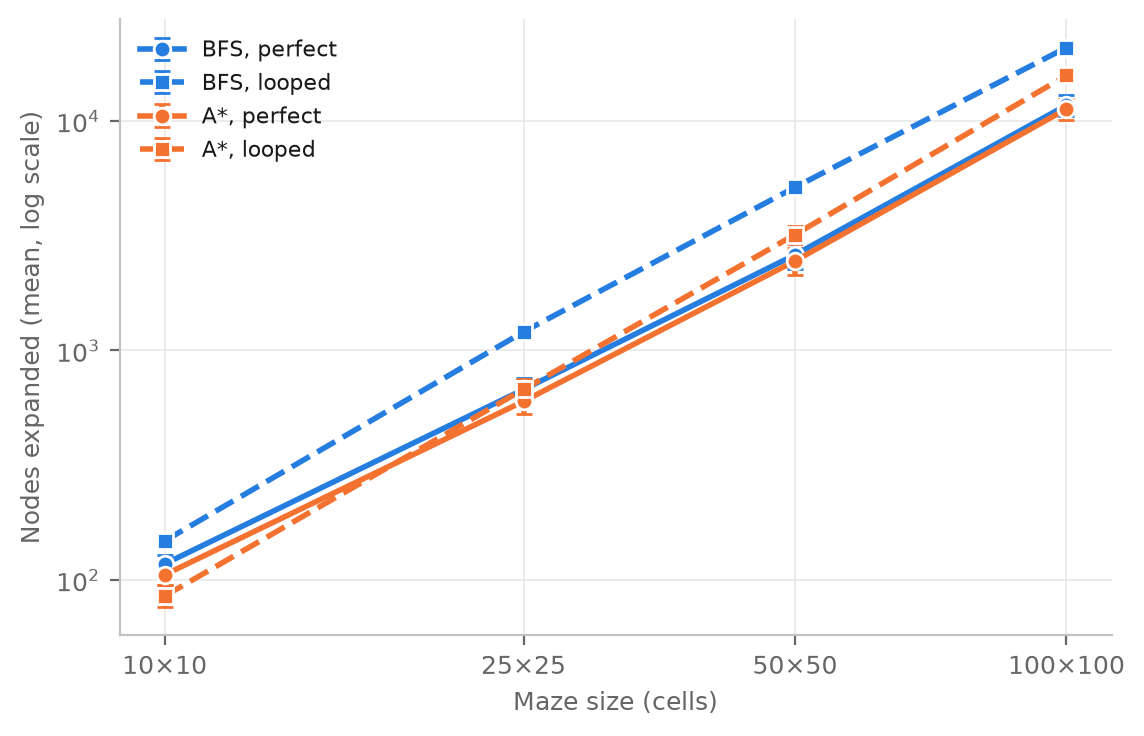
\includegraphics[width=\columnwidth]{figures/expanded_vs_size.png}
\caption{Nodes expanded against maze size for BFS and A* on perfect and looped mazes (final seeds 10000 to 10049, 50 mazes per point; both axes logarithmic; error bars are 95\% bootstrap confidence intervals of the mean and are mostly smaller than the markers).}
\label{fig:size}
\end{figure}

Fig.~\ref{fig:explore} shows why, on one typical 25$\times$25 seed. In the perfect maze (top row) the only route to the goal is 564 steps long although the goal is only 96 steps away in a straight line. A* expands 874 nodes against 964 for BFS: the heuristic prunes only a few side branches. In the looped maze of the same seed (bottom row) the shortest path drops to 160 steps, and A* leaves large regions untouched (689 expansions against 1,244).

\begin{figure*}[!t]
\centering
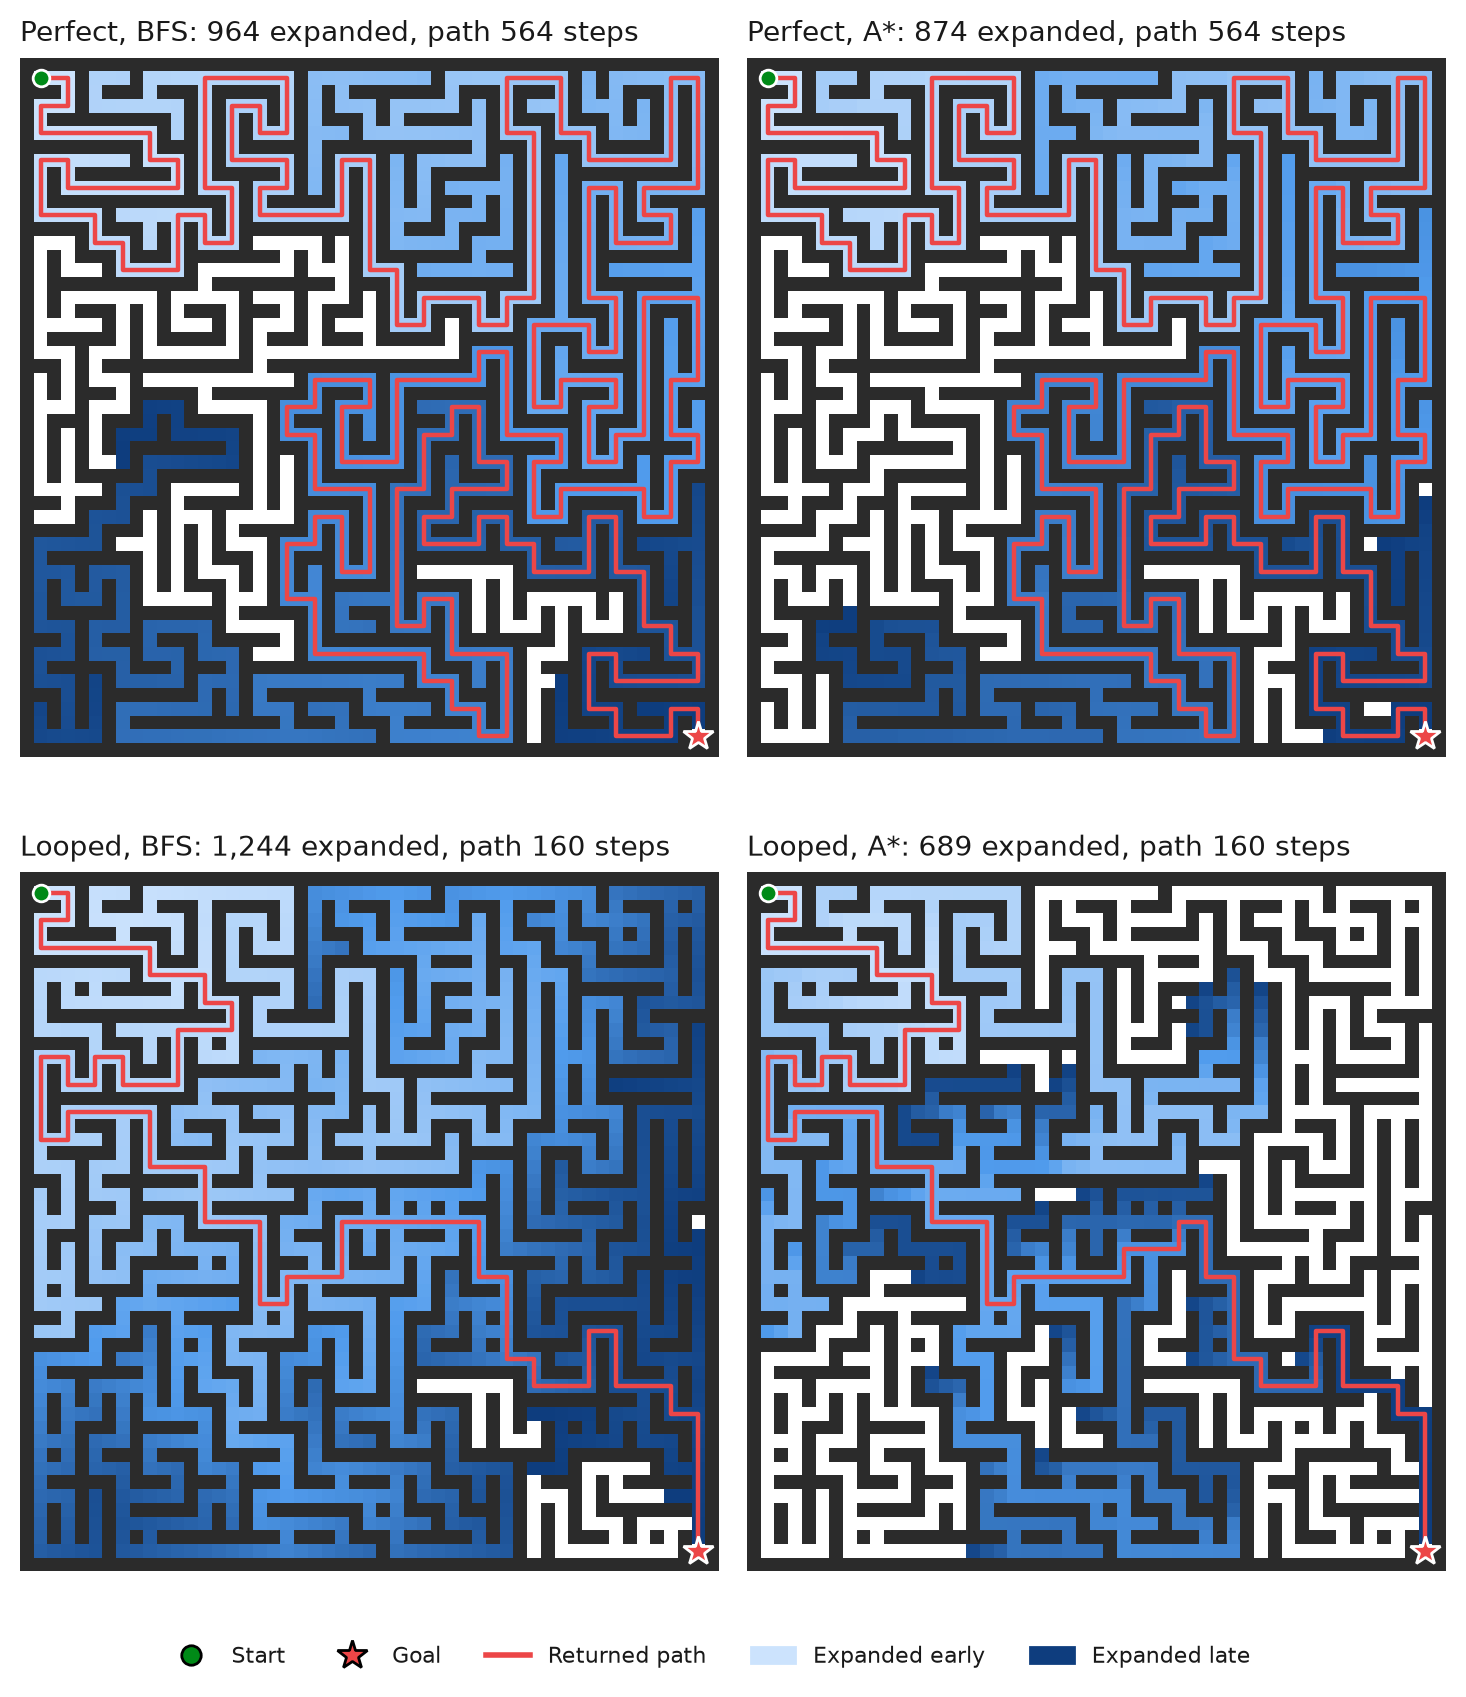
\includegraphics[width=0.91\textwidth]{figures/exploration_perfect_vs_looped.png}
\caption{BFS (left) and A* (right) on the same 25$\times$25 mazes: perfect (top) and looped with p = 0.1 (bottom), seed 10016. This seed was chosen by rule as the perfect maze whose savings are closest to the median. Squares are shaded by expansion order; white squares were never expanded.}
\label{fig:explore}
\end{figure*}

\subsection{The 30\% success criterion}
\begin{table*}[!t]
\centering
\footnotesize
\setlength{\tabw}{\dimexpr \textwidth-18\tabcolsep\relax}
\caption{Paired expansion savings of A* over BFS per maze (final seeds 10000 to 10049, 50 mazes per row). The target applies to 50$\times$50 and larger. Informedness is h(start)/C*.}
\label{tab:savings}
\begin{tabular}{>{\raggedright\arraybackslash}p{\dimexpr 0.0977\tabw\relax}>{\raggedright\arraybackslash}p{\dimexpr 0.0977\tabw\relax}>{\raggedleft\arraybackslash}p{\dimexpr 0.2069\tabw\relax}>{\raggedleft\arraybackslash}p{\dimexpr 0.0747\tabw\relax}>{\raggedleft\arraybackslash}p{\dimexpr 0.0805\tabw\relax}>{\raggedleft\arraybackslash}p{\dimexpr 0.1264\tabw\relax}>{\raggedleft\arraybackslash}p{\dimexpr 0.1264\tabw\relax}>{\raggedleft\arraybackslash}p{\dimexpr 0.0977\tabw\relax}>{\raggedleft\arraybackslash}p{\dimexpr 0.0920\tabw\relax}}
\toprule
\textbf{Maze type} & \textbf{Size} & \textbf{Mean savings [95\% CI]} & \textbf{SD} & \textbf{Median} & \textbf{Range} & \textbf{A* fewer / same / more} & \textbf{Mean informedness} & \textbf{$\geq$ 30\% target met} \\
\midrule
Perfect & 10$\times$10 & 10.2\% [8.3\%, 12.1\%] & 7.0\% & 9.6\% & 0\% to 29\% & 47 / 3 / 0 & 0.44 & n/a \\
Perfect & 25$\times$25 & 10.8\% [8.8\%, 12.9\%] & 7.4\% & 9.2\% & 0\% to 31\% & 49 / 1 / 0 & 0.26 & n/a \\
Perfect & 50$\times$50 & 6.3\% [5.2\%, 7.7\%] & 4.6\% & 5.2\% & 1\% to 24\% & 50 / 0 / 0 & 0.16 & No \\
Perfect & 100$\times$100 & 3.7\% [2.9\%, 4.6\%] & 3.1\% & 3.0\% & 0\% to 12\% & 50 / 0 / 0 & 0.09 & No \\
Looped & 10$\times$10 & 42.9\% [38.6\%, 47.2\%] & 15.6\% & 43.3\% & 1\% to 69\% & 50 / 0 / 0 & 0.74 & n/a \\
Looped & 25$\times$25 & 44.4\% [39.3\%, 49.5\%] & 18.5\% & 44.5\% & 1\% to 78\% & 50 / 0 / 0 & 0.73 & n/a \\
Looped & 50$\times$50 & 38.1\% [32.8\%, 43.5\%] & 19.5\% & 35.9\% & 3\% to 88\% & 50 / 0 / 0 & 0.73 & Yes \\
Looped & 100$\times$100 & 24.4\% [21.1\%, 27.8\%] & 12.2\% & 23.7\% & 6\% to 54\% & 50 / 0 / 0 & 0.74 & No \\
\bottomrule
\end{tabular}
\end{table*}

Table~\ref{tab:savings} answers the criterion separately for each size and type, as the proposal's wording requires, and Fig.~\ref{fig:box} shows the full distributions.

\begin{itemize}
  \item \textbf{Perfect mazes: the target is not met at either size.} Mean savings are 6.3\% [5.2\%, 7.7\%] at 50$\times$50 and 3.7\% [2.9\%, 4.6\%] at 100$\times$100. The upper ends of the confidence intervals are far below 30\%, so this is not a borderline miss.
  \item \textbf{Looped mazes: the target is met at 50$\times$50 (38.1\% [32.8\%, 43.5\%]) and not met at 100$\times$100 (24.4\% [21.1\%, 27.8\%]).} The confidence intervals show how close each case is to the 30\% line; where an interval contains 30\%, the verdict should be read as marginal rather than decisive.
\end{itemize}

We report this as it is: the criterion in the proposal is only partly met. A* expanded fewer nodes than BFS on 396 of the 400 mazes, the same number on 4, and more on 0, and the Wilcoxon test rejects ``no difference'' in every row (largest p-value 1.2e-09). So A* is reliably \emph{no worse} than BFS, but ``reliably fewer'' and ``30\% fewer'' are very different claims. Averages also hide a wide spread: on looped mazes individual savings range from 1\% to 88\%. The ratio of mean expansions, an alternative reading of ``on average'', gives the same verdicts (5.9\% and 3.7\% for perfect, 37.8\% and 24.4\% for looped mazes).

\begin{figure}[!t]
\centering
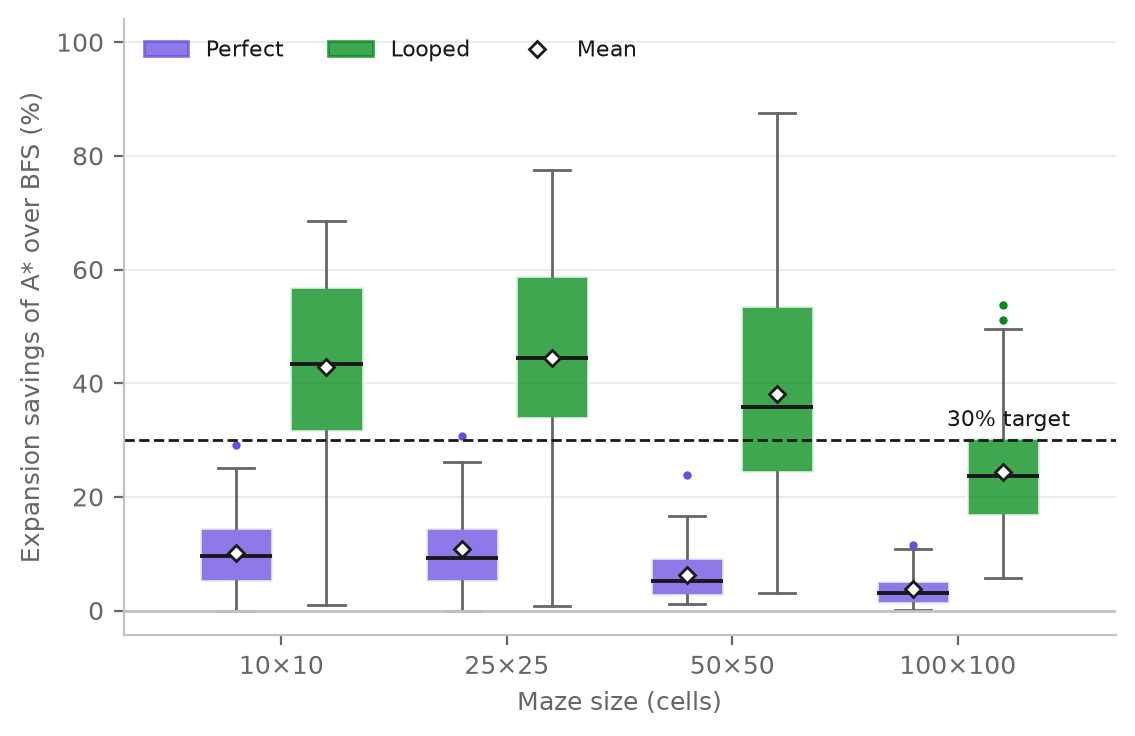
\includegraphics[width=\columnwidth]{figures/savings_by_size_and_type.png}
\caption{Distribution of per-maze expansion savings of A* over BFS (final seeds 10000 to 10049, 50 mazes per box). Boxes span the quartiles, the line is the median, the diamond is the mean, whiskers reach 1.5 times the interquartile range, and dots are individual mazes beyond them. The dashed line is the 30\% target.}
\label{fig:box}
\end{figure}

Two trends in Table~\ref{tab:savings} need explaining. First, perfect mazes get \emph{worse} for A* as they grow: savings fall from 10.2\% at 10$\times$10 to 3.7\% at 100$\times$100. The informedness column shows why. The depth-first generator makes solution paths that wind more and more as the maze grows, so the straight-line estimate at the start covers 44\% of the true distance at 10$\times$10 but only 9\% at 100$\times$100. Second, looped mazes also lose savings with size (44.4\% at 25$\times$25, 24.4\% at 100$\times$100) even though their mean informedness stays near 0.74. A likely reason is that what A* can prune is governed by the absolute slack C* $-$ h(start), not the ratio: A* must expand every node with g + h \textless{} C*, and a slack of a quarter of the path length is a few dozen steps in a small maze but several hundred steps in a large one, enough to reach into most side regions whose local detours have a fixed size. We did not test this explanation directly.


\subsection{When does the heuristic stop helping? (RQ2)}

To answer the title question we varied one thing, the loop rate p, from 0 (a perfect maze) to 1 (every internal wall removed, an open grid with pillars), on fresh seeds (20000 to 20049), and ran BFS and A* with both tie rules on every maze. Fig.~\ref{fig:sweep} and Table~\ref{tab:sweep} show the result.

\begin{table*}[!t]
\centering
\footnotesize
\setlength{\tabw}{\dimexpr \textwidth-16\tabcolsep\relax}
\caption{Loop rate sweep: mean expansion savings of A* over BFS for the two tie rules (final seeds 20000 to 20049, 50 mazes per cell, nested mazes per seed). Informedness is the mean h(start)/C* at 50$\times$50.}
\label{tab:sweep}
\begin{tabular}{>{\raggedright\arraybackslash}p{\dimexpr 0.1030\tabw\relax}>{\raggedleft\arraybackslash}p{\dimexpr 0.1333\tabw\relax}>{\raggedleft\arraybackslash}p{\dimexpr 0.1273\tabw\relax}>{\raggedleft\arraybackslash}p{\dimexpr 0.1273\tabw\relax}>{\raggedleft\arraybackslash}p{\dimexpr 0.1273\tabw\relax}>{\raggedleft\arraybackslash}p{\dimexpr 0.1273\tabw\relax}>{\raggedleft\arraybackslash}p{\dimexpr 0.1273\tabw\relax}>{\raggedleft\arraybackslash}p{\dimexpr 0.1273\tabw\relax}}
\toprule
\textbf{Loop rate p} & \textbf{Informedness (50$\times$50)} & \textbf{Larger-g, 25$\times$25} & \textbf{Larger-g, 50$\times$50} & \textbf{Larger-g, 100$\times$100} & \textbf{FIFO, 25$\times$25} & \textbf{FIFO, 50$\times$50} & \textbf{FIFO, 100$\times$100} \\
\midrule
0 & 0.15 & 8\% & 6\% & 3\% & 7\% & 6\% & 3\% \\
0.02 & 0.37 & 23\% & 21\% & 14\% & 21\% & 21\% & 13\% \\
0.05 & 0.56 & 31\% & 26\% & 19\% & 28\% & 25\% & 18\% \\
0.1 & 0.72 & 46\% & 33\% & 29\% & 40\% & 30\% & 27\% \\
0.2 & 0.90 & 62\% & 65\% & 58\% & 51\% & 56\% & 53\% \\
0.35 & 0.99 & 81\% & 87\% & 90\% & 58\% & 66\% & 73\% \\
0.5 & 1.00 & 87\% & 89\% & 91\% & 35\% & 41\% & 43\% \\
0.75 & 1.00 & 91\% & 93\% & 95\% & 12\% & 13\% & 14\% \\
1 & 1.00 & 95\% & 97\% & 99\% & 0\% & 0\% & 0\% \\
\bottomrule
\end{tabular}
\end{table*}
\begin{figure*}[!t]
\centering
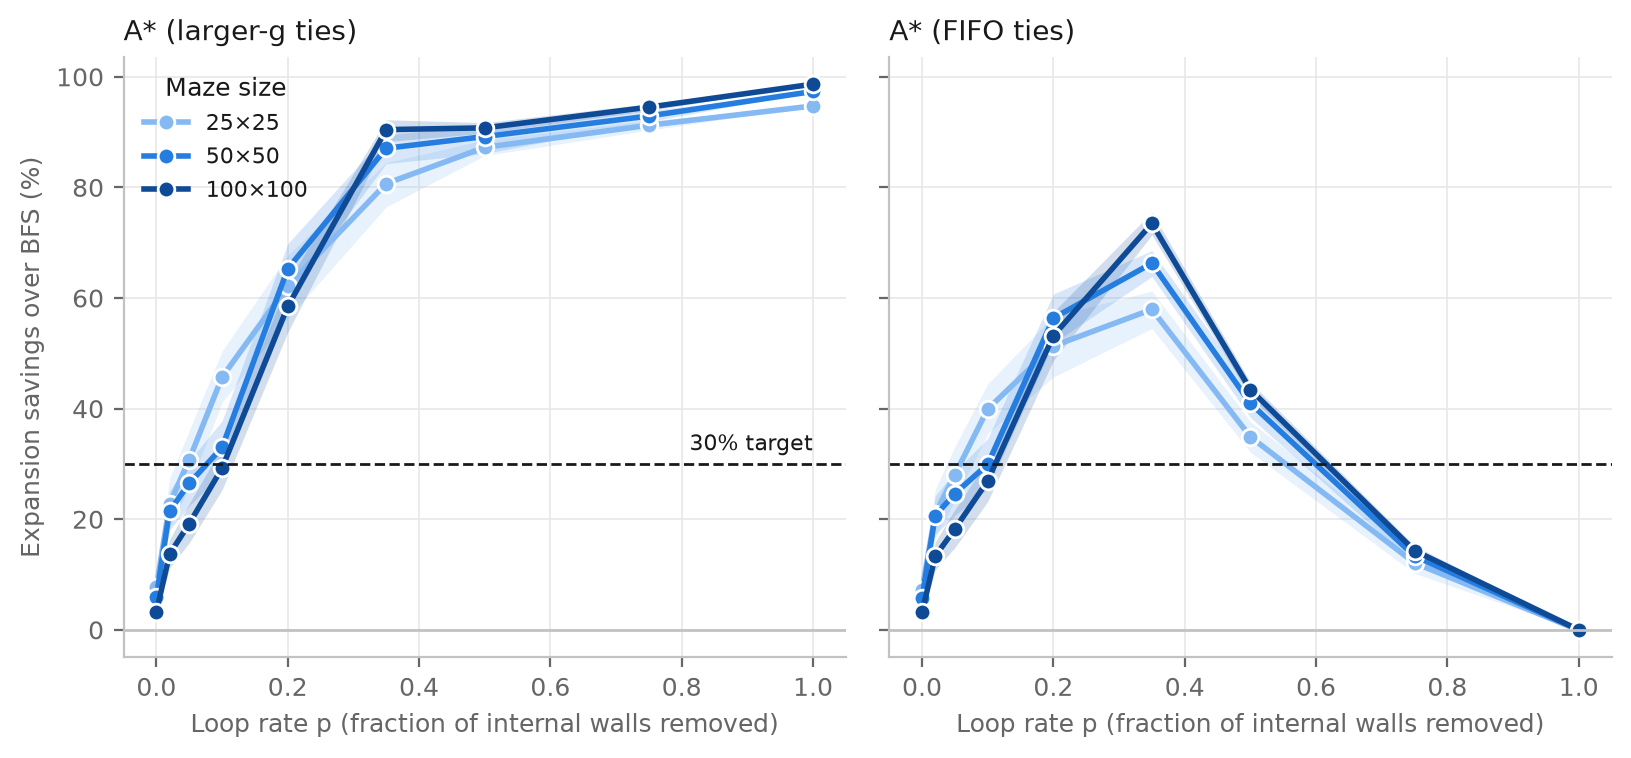
\includegraphics[width=0.97\textwidth]{figures/savings_vs_loop_rate.png}
\caption{Mean expansion savings of A* over BFS as walls are removed, for larger-g ties (left) and FIFO ties (right). Final seeds 20000 to 20049, 50 mazes per point; bands are 95\% bootstrap confidence intervals; the dashed line is the 30\% target.}
\label{fig:sweep}
\end{figure*}

\textbf{Finding 1: the heuristic helps in proportion to how informed it is.} With larger-g ties, savings rise steadily with p: 6\% at p = 0, 33\% at p = 0.1, 87\% at p = 0.35 and 97\% at p = 1 (50$\times$50). Removing walls shortens the true route toward the straight-line distance, so h approaches h* and the set of nodes with f \textless{} C* that A* is forced to expand shrinks. Fig.~\ref{fig:informed} plots every maze of the sweep by its informedness. The relationship is strong for larger-g ties (Spearman rank correlation 0.92; only 0.19 for FIFO ties, for the reason given in Finding 2) and Table~\ref{tab:bins} turns it into a rule of thumb: when h(start)/C* is below 0.4, A* reached the 30\% target on only 13 of 248 mazes; when it is above 0.9, on 686 of 686.

\begin{figure*}[!t]
\centering
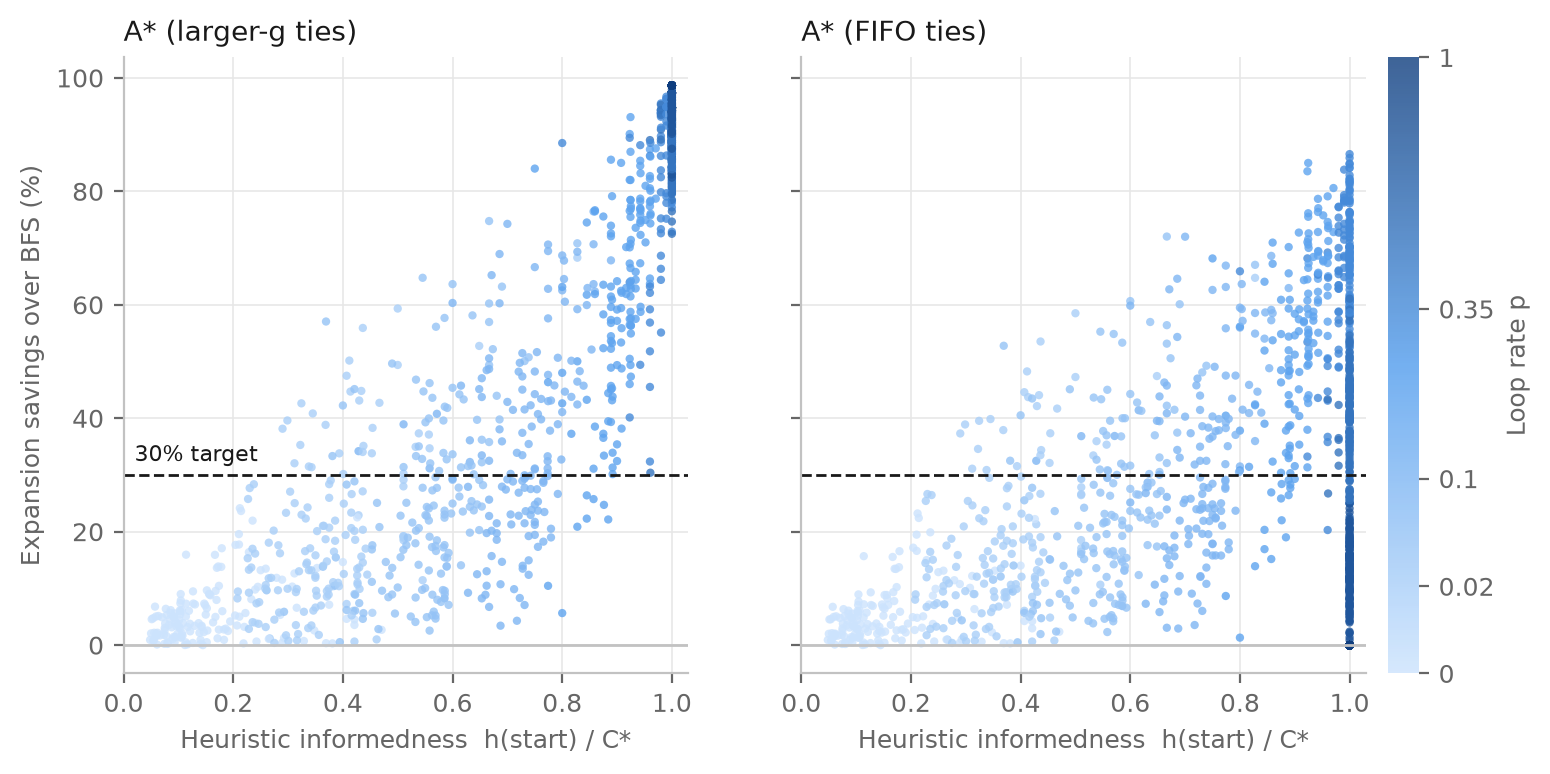
\includegraphics[width=0.97\textwidth]{figures/savings_vs_informedness.png}
\caption{Expansion savings against heuristic informedness h(start)/C*, one dot per maze of the sweep (1,350 mazes: 25$\times$25, 50$\times$50 and 100$\times$100, nine loop rates, final seeds 20000 to 20049). Colour is the loop rate. Left: larger-g ties. Right: FIFO ties, where savings collapse on the mazes with informedness 1.}
\label{fig:informed}
\end{figure*}
\begin{table*}[!t]
\centering
\footnotesize
\setlength{\tabw}{\dimexpr \textwidth-12\tabcolsep\relax}
\caption{Savings grouped by heuristic informedness, all sizes and loop rates of the sweep pooled (final seeds 20000 to 20049). The last row holds the mazes in which the Manhattan distance from the start is exact.}
\label{tab:bins}
\begin{tabular}{>{\raggedright\arraybackslash}p{\dimexpr 0.2250\tabw\relax}>{\raggedleft\arraybackslash}p{\dimexpr 0.1000\tabw\relax}>{\raggedleft\arraybackslash}p{\dimexpr 0.1688\tabw\relax}>{\raggedleft\arraybackslash}p{\dimexpr 0.1688\tabw\relax}>{\raggedleft\arraybackslash}p{\dimexpr 0.1688\tabw\relax}>{\raggedleft\arraybackslash}p{\dimexpr 0.1688\tabw\relax}}
\toprule
\textbf{Informedness h(start)/C*} & \textbf{Mazes} & \textbf{Larger-g: mean savings} & \textbf{Larger-g: mazes $\geq$ 30\%} & \textbf{FIFO: mean savings} & \textbf{FIFO: mazes $\geq$ 30\%} \\
\midrule
0.0 to 0.1 & 43 & 3\% & 0 & 3\% & 0 \\
0.1 to 0.2 & 66 & 5\% & 0 & 5\% & 0 \\
0.2 to 0.3 & 63 & 12\% & 2 & 11\% & 2 \\
0.3 to 0.4 & 76 & 16\% & 11 & 15\% & 10 \\
0.4 to 0.5 & 72 & 20\% & 17 & 19\% & 16 \\
0.5 to 0.6 & 100 & 25\% & 32 & 23\% & 28 \\
0.6 to 0.7 & 73 & 33\% & 38 & 30\% & 32 \\
0.7 to 0.8 & 93 & 35\% & 50 & 31\% & 43 \\
0.8 to 0.9 & 78 & 52\% & 72 & 45\% & 64 \\
0.9 to \textless{}1.0 & 138 & 74\% & 138 & 61\% & 136 \\
1.0 & 548 & 92\% & 548 & 27\% & 226 \\
\bottomrule
\end{tabular}
\end{table*}

\textbf{Finding 2: an exact heuristic is still not enough; tie-breaking decides.} With FIFO ties the curve in Fig.~\ref{fig:sweep} is not monotone. Savings peak near p = 0.35 (66\% at 50$\times$50) and then fall, reaching 0.0\% at p = 1, where A* with FIFO ties expanded \emph{more} nodes than BFS on all 150 mazes (by exactly 1 node). On those mazes the heuristic is perfect at the start. The explanation is the f = C* plateau from Section II-B: on an open grid a very large number of squares lie on some shortest path, and every one of them has f = C* exactly. A consistent heuristic tells A* nothing about the order within a plateau. FIFO ties sweep it level by level, exactly like BFS, and BFS even stops slightly earlier because it tests the goal at generation. Preferring the larger g dives along one shortest path and saves 97\%. The hand-traced 3$\times$3 open grid in our tests shows the same effect in miniature (7 expansions for BFS, 8 for A* with FIFO ties, 4 with larger-g ties). This is the same path symmetry that Jump Point Search was designed to remove~\cite{ref8}.


\textbf{Answer to the title question.} The Manhattan heuristic stops helping in two different regimes. In tree-like mazes it is \emph{uninformed}: the true route is several times longer than the straight line, most nodes have f \textless{} C*, and A* is forced to expand them, dead ends included. On open grids it is \emph{uninformative among ties}: it is exact, but so many nodes share f = C* that the result depends on tie-breaking rather than on the heuristic. The best case for A* lies between the two, or anywhere on the open side with a tie rule that prefers depth. The single quantity h(start)/C* predicts the first regime well; it cannot see the second.


\subsection{A worked failure case}

Fig.~\ref{fig:failure} shows the maze with the lowest savings among the 25$\times$25 mazes of the main experiment (perfect, seed 10029). A* expanded 342 nodes and BFS 342, a saving of 0.0\%. The shortest path is 268 steps although the Manhattan distance is 96, an informedness of 0.36. The mechanism can be read off f = g + h. The goal has f = C* = 268. Any square x that can be reached in g(x) steps has f(x) = g(x) + h(x), and h(x) is at most 96, so every square that can be reached in fewer than 172 steps has f \textless{} C* no matter where it lies, and A* is obliged to expand it before it may stop. In this maze the branches off the solution path are short dead-end pockets, so everything BFS reaches before it finds the goal is inside that budget, and the two algorithms expand exactly the same squares. The dead ends pointing toward the goal, which our proposal expected to hurt A*, are indeed expanded early because their h is small. But the deeper problem is the length of the detour itself: when the route is several times longer than the straight line, the heuristic's opinion about direction is worth almost nothing. A* tied with BFS in this way on 4 of the 400 mazes of the main experiment, all of them perfect mazes, and never expanded more.

\begin{figure*}[!t]
\centering
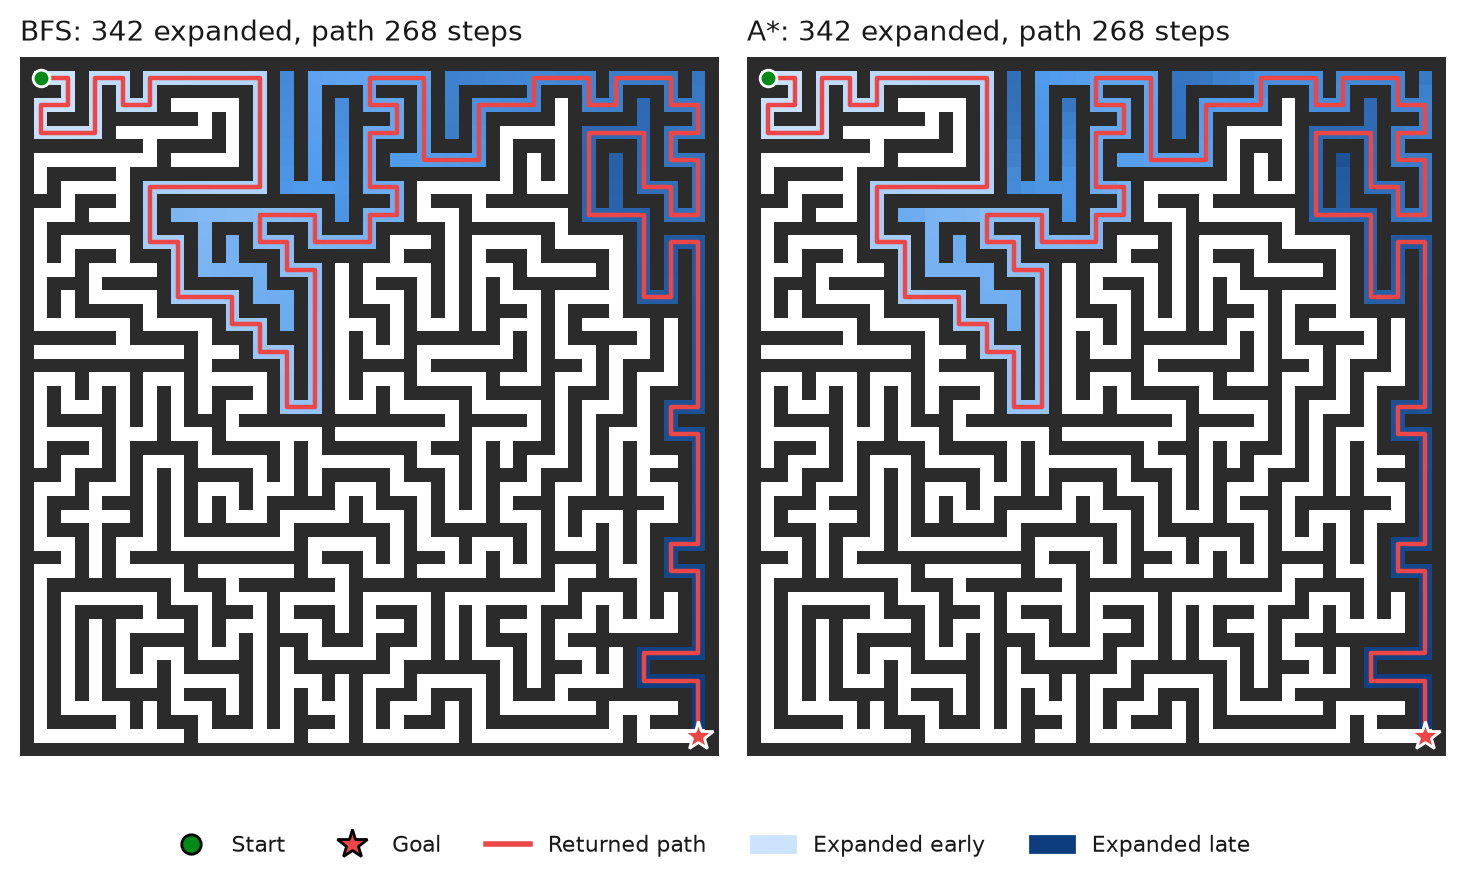
\includegraphics[width=0.91\textwidth]{figures/failure_case.png}
\caption{Failure case: the 25$\times$25 maze of the main experiment with the lowest savings (perfect, seed 10029). BFS (left) and A* (right) expand exactly the same squares: the route is so much longer than the straight-line distance that every square near it has f below C*.}
\label{fig:failure}
\end{figure*}

\subsection{Weighted mazes: UCS, A* and BFS (RQ3)}

In weighted mazes the baseline is UCS, as stated in the proposal, and BFS is kept as a reference that optimizes the wrong objective. Mazes are looped (p = 0.1) with a fraction m of muddy squares, on fresh seeds (21000 to 21049); Table~\ref{tab:weighted} and Fig.~\ref{fig:weighted} summarize the results.

\begin{table*}[!t]
\centering
\footnotesize
\setlength{\tabw}{\dimexpr \textwidth-18\tabcolsep\relax}
\caption{Weighted extension (looped mazes with p = 0.1, mud costs 5; final seeds 21000 to 21049, 50 mazes per row). Savings are paired per maze. ``Extra cost'' is the cost of the BFS path relative to the optimal cost. Informedness is h(start)/C* with C* the optimal cost.}
\label{tab:weighted}
\begin{tabular}{>{\raggedright\arraybackslash}p{\dimexpr 0.0914\tabw\relax}>{\raggedleft\arraybackslash}p{\dimexpr 0.0800\tabw\relax}>{\raggedleft\arraybackslash}p{\dimexpr 0.1029\tabw\relax}>{\raggedleft\arraybackslash}p{\dimexpr 0.1029\tabw\relax}>{\raggedleft\arraybackslash}p{\dimexpr 0.2114\tabw\relax}>{\raggedleft\arraybackslash}p{\dimexpr 0.1029\tabw\relax}>{\raggedleft\arraybackslash}p{\dimexpr 0.0971\tabw\relax}>{\raggedleft\arraybackslash}p{\dimexpr 0.0971\tabw\relax}>{\raggedleft\arraybackslash}p{\dimexpr 0.1143\tabw\relax}}
\toprule
\textbf{Size} & \textbf{Mud rate m} & \textbf{UCS expanded} & \textbf{A* expanded} & \textbf{A* savings over UCS [95\% CI]} & \textbf{Informedness} & \textbf{BFS extra cost, mean} & \textbf{BFS extra cost, max} & \textbf{Mazes where BFS is not optimal} \\
\midrule
25$\times$25 & 0 & 1,201 & 705 & 42.0\% [37.3\%, 46.7\%] & 0.72 & 0.0\% & 0.0\% & 0 / 50 \\
25$\times$25 & 0.1 & 1,179 & 862 & 27.9\% [23.4\%, 32.3\%] & 0.55 & 3.8\% & 17.4\% & 36 / 50 \\
25$\times$25 & 0.2 & 1,176 & 956 & 19.6\% [16.2\%, 23.1\%] & 0.43 & 3.8\% & 14.6\% & 39 / 50 \\
25$\times$25 & 0.4 & 1,191 & 1,075 & 10.3\% [8.2\%, 12.6\%] & 0.29 & 2.5\% & 11.5\% & 34 / 50 \\
50$\times$50 & 0 & 5,173 & 3,304 & 36.2\% [31.7\%, 40.6\%] & 0.72 & 0.0\% & 0.0\% & 0 / 50 \\
50$\times$50 & 0.1 & 5,148 & 4,180 & 18.9\% [15.2\%, 22.9\%] & 0.54 & 4.3\% & 12.5\% & 45 / 50 \\
50$\times$50 & 0.2 & 5,143 & 4,627 & 10.1\% [8.0\%, 12.5\%] & 0.42 & 5.6\% & 17.7\% & 46 / 50 \\
50$\times$50 & 0.4 & 5,154 & 4,922 & 4.5\% [3.4\%, 5.8\%] & 0.29 & 4.2\% & 11.5\% & 47 / 50 \\
100$\times$100 & 0 & 20,939 & 16,432 & 21.5\% [18.4\%, 25.0\%] & 0.75 & 0.0\% & 0.0\% & 0 / 50 \\
100$\times$100 & 0.1 & 20,923 & 19,352 & 7.5\% [5.9\%, 9.5\%] & 0.56 & 5.7\% & 16.8\% & 50 / 50 \\
100$\times$100 & 0.2 & 20,919 & 20,272 & 3.1\% [2.1\%, 4.5\%] & 0.44 & 5.9\% & 13.4\% & 50 / 50 \\
100$\times$100 & 0.4 & 20,911 & 20,655 & 1.2\% [0.7\%, 1.9\%] & 0.30 & 5.2\% & 13.6\% & 50 / 50 \\
\bottomrule
\end{tabular}
\end{table*}

\textbf{UCS and A* agree; A* does less work, but less than before.} UCS and A* returned the same optimal cost on all 600 of 600 weighted-experiment mazes. A* expanded fewer nodes than UCS, but its advantage shrinks quickly as mud is added: at 100$\times$100 from 21.5\% with no mud to 3.1\% at m = 0.2 and 1.2\% at m = 0.4. This is the informedness effect again. Mud raises the true cost of every route, but Manhattan distance must assume that every remaining square costs 1, so h falls further below h* (the informedness column drops from 0.75 to 0.30). The heuristic is still admissible and consistent, and A* is still optimal; it is simply a looser bound.


\textbf{BFS is wrong, moderately and often.} BFS still returns a path with the fewest steps, but with mud that is no longer the cheapest path. At the default m = 0.2 the BFS path cost more than the optimum on 39 of 50 mazes at 25$\times$25, 46 of 50 mazes at 50$\times$50, 50 of 50 mazes at 100$\times$100, by 3.8\% to 5.9\% on average and by up to 17.7\% on a single maze. Fig.~\ref{fig:wpaths} shows the maze with the largest gap at 25$\times$25: BFS returns a path of 128 steps that costs 220, while UCS and A* return a path of 132 steps that costs 192. Fewest actions is not lowest cost. BFS also expands about as many nodes as UCS, so in a weighted maze it is neither cheaper to run nor correct.

\begin{figure*}[!t]
\centering
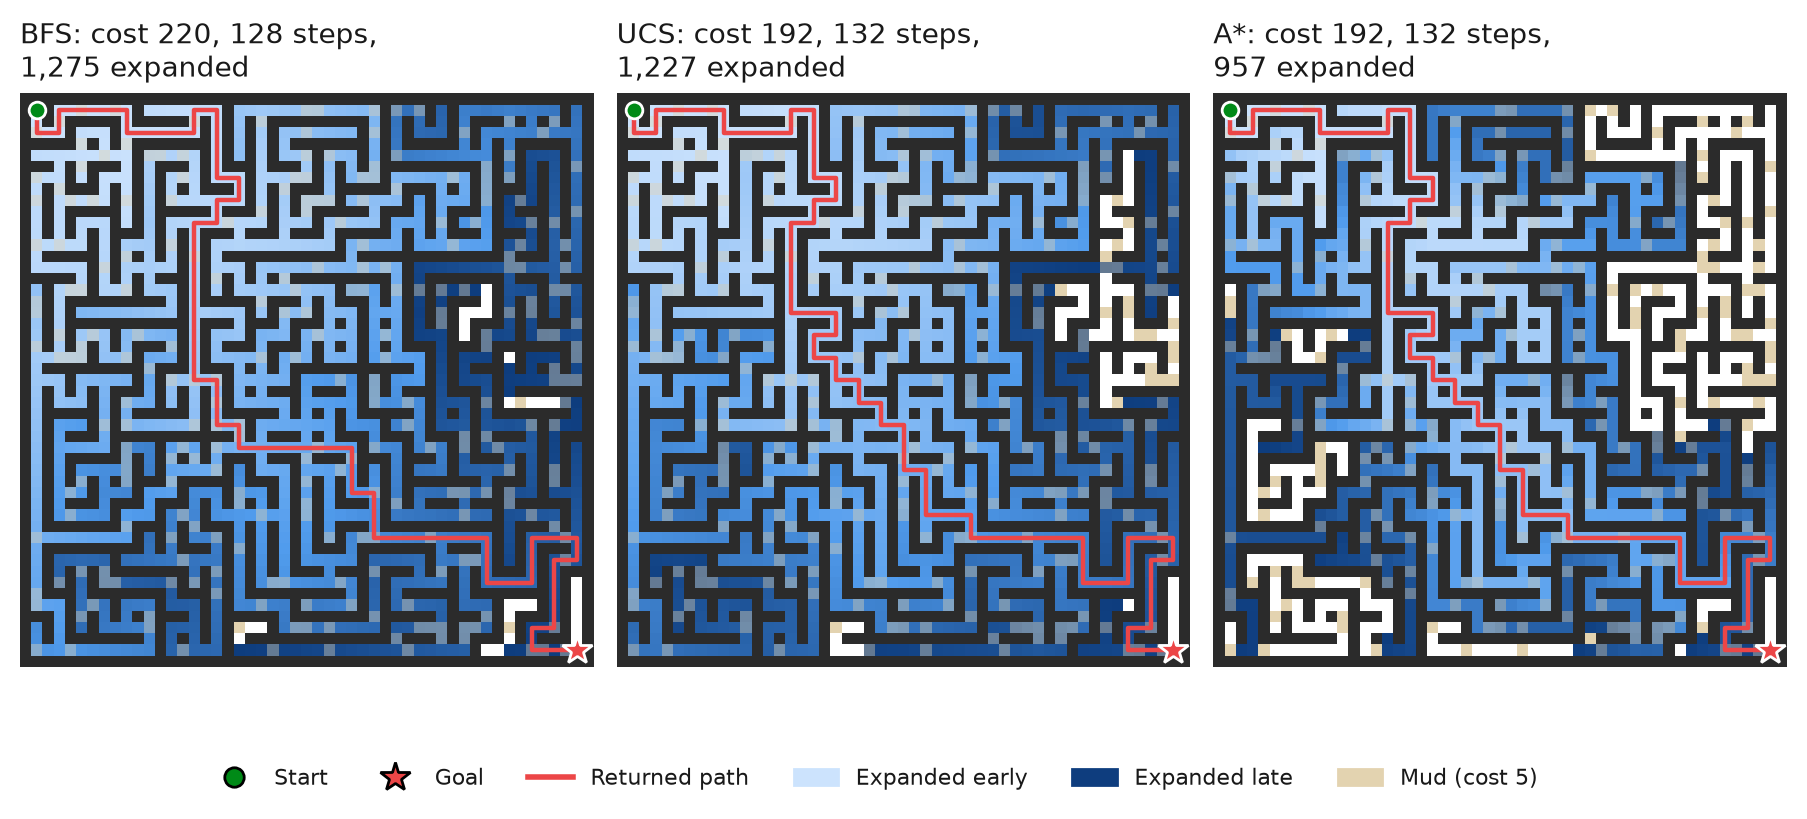
\includegraphics[width=1.00\textwidth]{figures/weighted_paths.png}
\caption{A weighted 25$\times$25 maze (p = 0.1, m = 0.2, seed 21036; chosen by rule as the 25$\times$25 maze with the largest extra cost for BFS). Mud squares are tan. BFS minimizes steps and pays more; UCS and A* return the same optimal cost, and A* expands fewer nodes.}
\label{fig:wpaths}
\end{figure*}
\begin{figure*}[!t]
\centering
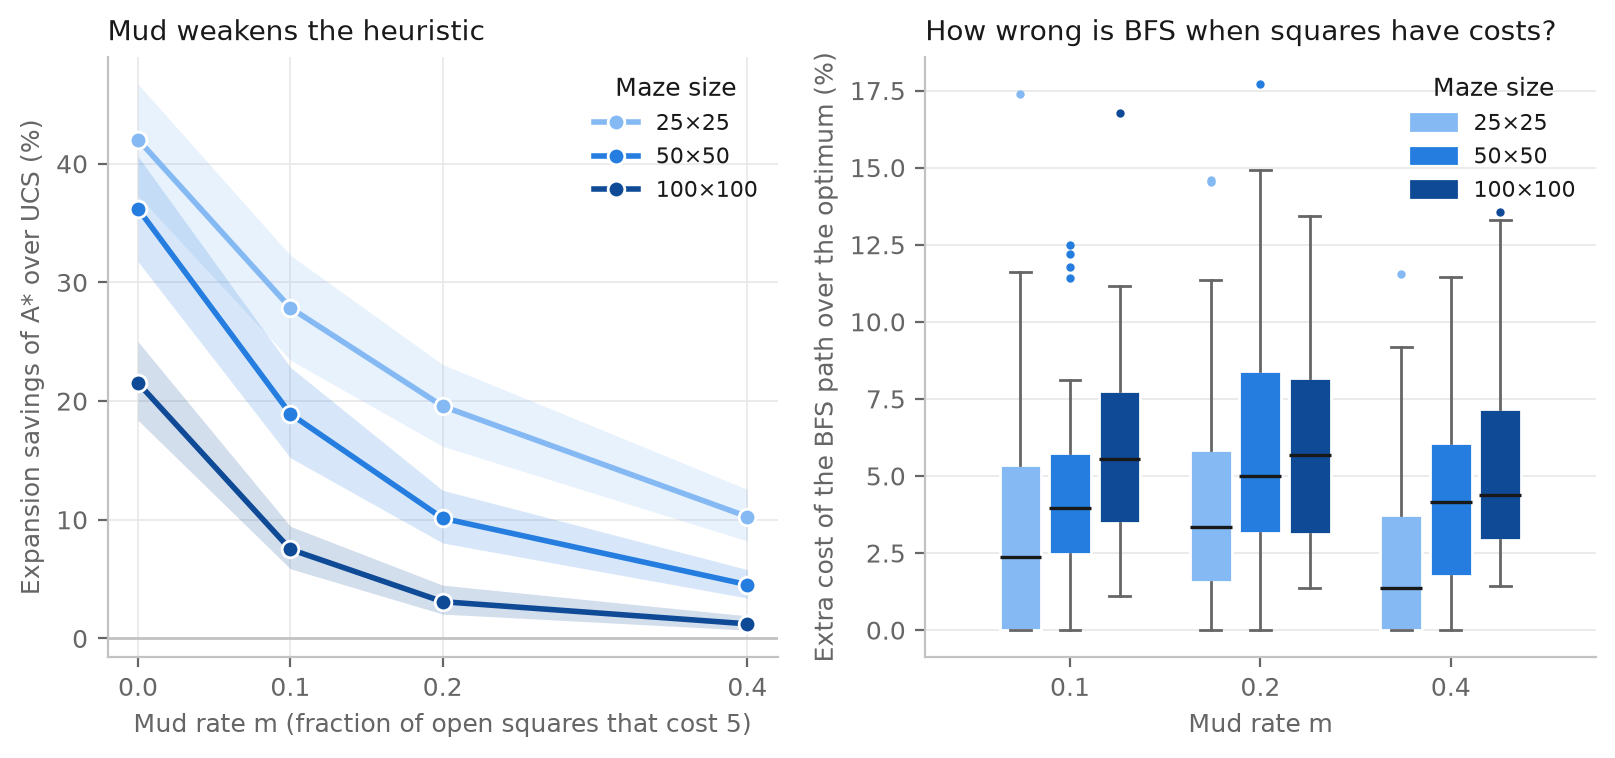
\includegraphics[width=0.97\textwidth]{figures/weighted_extension.png}
\caption{Weighted extension (final seeds 21000 to 21049, 50 mazes per point or box). Left: mean paired expansion savings of A* over UCS against the mud rate, with 95\% bootstrap bands. Right: extra cost of the BFS path over the optimal cost.}
\label{fig:weighted}
\end{figure*}

\subsection{Ablations}

The ablations use their own seeds (22000 to 22049) and nine configurations on the same mazes. Table~\ref{tab:ablation} lists the 100$\times$100 results and Fig.~\ref{fig:ablation} plots the savings.

\begin{table*}[!t]
\centering
\footnotesize
\setlength{\tabw}{\dimexpr \textwidth-18\tabcolsep\relax}
\caption{Ablations on 100$\times$100 mazes (final seeds 22000 to 22049, 50 perfect and 50 looped mazes, p = 0.1). Savings are the mean of the paired per-maze savings relative to BFS with the goal test at generation. ``Optimal'' counts mazes on which the returned path was a shortest path; ``extra path cost'' is the mean excess over the optimum.}
\label{tab:ablation}
\begin{tabular}{>{\raggedright\arraybackslash}p{\dimexpr 0.2222\tabw\relax}>{\raggedleft\arraybackslash}p{\dimexpr 0.1049\tabw\relax}>{\raggedleft\arraybackslash}p{\dimexpr 0.0988\tabw\relax}>{\raggedleft\arraybackslash}p{\dimexpr 0.0926\tabw\relax}>{\raggedleft\arraybackslash}p{\dimexpr 0.0926\tabw\relax}>{\raggedleft\arraybackslash}p{\dimexpr 0.1049\tabw\relax}>{\raggedleft\arraybackslash}p{\dimexpr 0.0988\tabw\relax}>{\raggedleft\arraybackslash}p{\dimexpr 0.0926\tabw\relax}>{\raggedleft\arraybackslash}p{\dimexpr 0.0926\tabw\relax}}
\toprule
\textbf{Configuration} & \textbf{Perfect: expanded} & \textbf{Savings vs BFS} & \textbf{Optimal} & \textbf{Extra path cost} & \textbf{Looped: expanded} & \textbf{Savings vs BFS} & \textbf{Optimal} & \textbf{Extra path cost} \\
\midrule
BFS & 10,186 & baseline & 50 / 50 & 0.0\% & 20,917 & baseline & 50 / 50 & 0.0\% \\
BFS (goal test at removal) & 10,190 & 0.0\% & 50 / 50 & 0.0\% & 20,922 & 0.0\% & 50 / 50 & 0.0\% \\
A* (h = 0) & 10,190 & 0.0\% & 50 / 50 & 0.0\% & 20,922 & 0.0\% & 50 / 50 & 0.0\% \\
A* (FIFO ties) & 9,760 & 4.3\% & 50 / 50 & 0.0\% & 16,608 & 20.6\% & 50 / 50 & 0.0\% \\
A* (larger-g ties) & 9,751 & 4.4\% & 50 / 50 & 0.0\% & 16,221 & 22.5\% & 50 / 50 & 0.0\% \\
Weighted A* (w = 1.5) & 9,603 & 5.9\% & 50 / 50 & 0.0\% & 3,006 & 85.6\% & 10 / 50 & 2.8\% \\
Weighted A* (w = 2) & 9,426 & 7.7\% & 50 / 50 & 0.0\% & 1,632 & 92.2\% & 1 / 50 & 10.7\% \\
Weighted A* (w = 3) & 9,111 & 10.6\% & 50 / 50 & 0.0\% & 1,357 & 93.5\% & 0 / 50 & 18.9\% \\
Greedy & 6,603 & 34.7\% & 50 / 50 & 0.0\% & 1,056 & 95.0\% & 0 / 50 & 38.8\% \\
\bottomrule
\end{tabular}
\end{table*}
\begin{itemize}
  \item \textbf{BFS goal test timing.} Testing the goal at removal instead of at generation costs BFS 4.6 extra expansions per maze on average, which is negligible at these sizes. The definition of the baseline therefore does not drive the 30\% verdicts, but we kept the stronger baseline for the headline numbers.
  \item \textbf{A* with h = 0.} It expands exactly as many nodes as BFS with the goal test at removal in every row of Table~\ref{tab:ablation}: with unit costs, UCS is BFS. All the benefit of A* comes from the heuristic.
  \item \textbf{Tie rule.} At the default p = 0.1 the tie rule matters little: larger-g ties save 22.5\% and FIFO ties 20.6\% on looped mazes, and they are within 0.1 percentage points of each other on perfect mazes. The large effect appears only at high loop rates (Section IV-C), where f = C* plateaus are large.
  \item \textbf{Greedy best-first and weighted A*.} On looped mazes greedy search expands 95\% fewer nodes than BFS, far more than A*, but its path was optimal on only 0 of 50 mazes and was 38.8\% longer on average. Weighted A* sits between: with w = 1.5 it saves 86\% for paths 2.8\% longer, and with w = 2, 92\% for 10.7\%. Fewer expansions alone do not establish a better solution. On perfect mazes both remain optimal on every maze (50 of 50 for greedy), simply because there is only one route to return; this is the same reason we did not build weighted mazes on perfect mazes.
\end{itemize}
\begin{figure*}[!t]
\centering
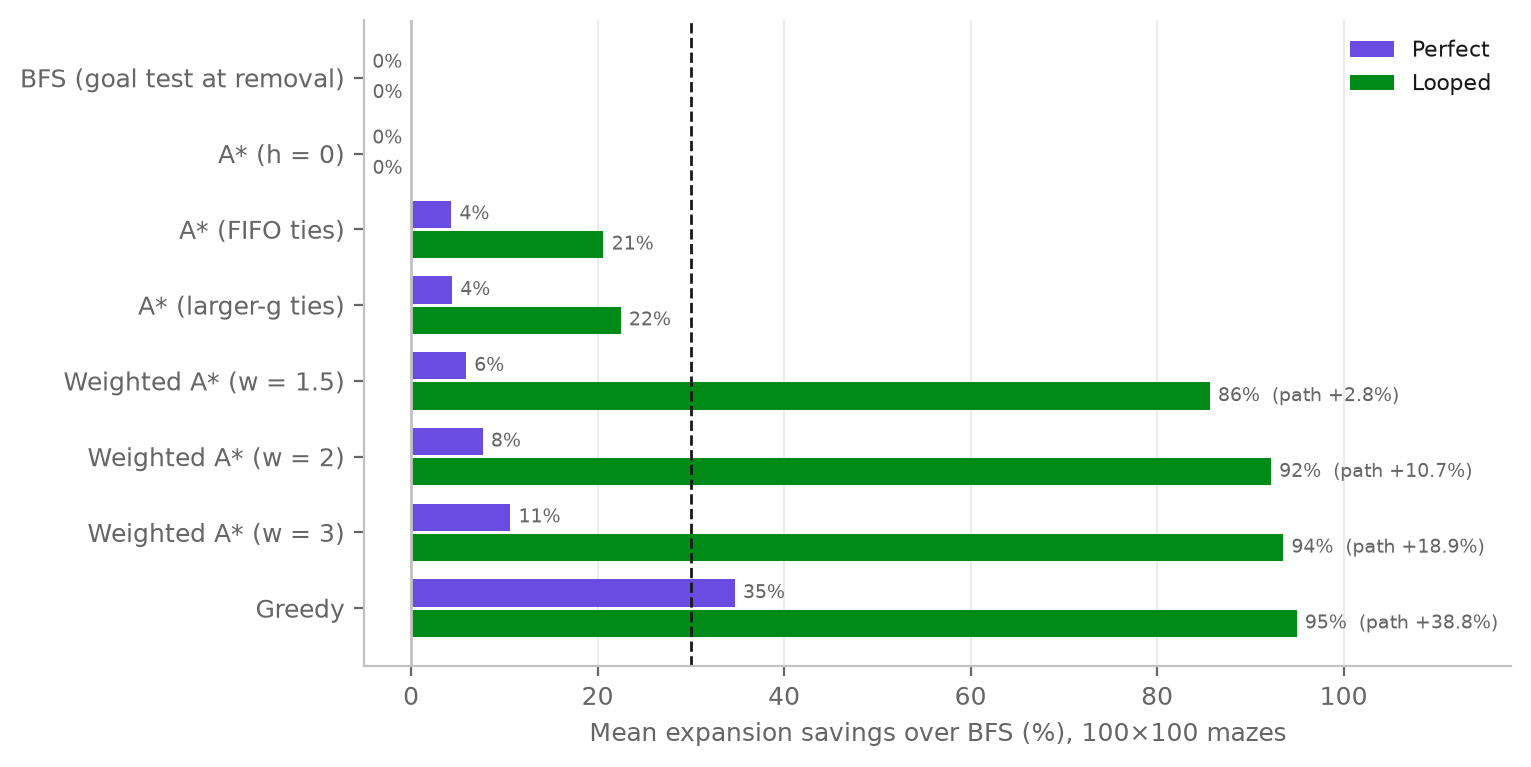
\includegraphics[width=0.84\textwidth]{figures/ablation.png}
\caption{Mean paired expansion savings over BFS for each ablation configuration on 100$\times$100 mazes (final seeds 22000 to 22049, 50 mazes per bar). Labels in parentheses give the mean extra path cost where the returned paths were not all optimal. The dashed line is the 30\% target, which applies to optimal algorithms only.}
\label{fig:ablation}
\end{figure*}

\subsection{Runtime and memory}

Runtime tells a more sober story than expansions (Fig.~\ref{fig:runtime}). A* was faster than BFS on only 101 of the 400 mazes of the main experiment. At 100$\times$100 it took 15.4 ms against 11.7 ms for BFS on perfect mazes and 26.6 ms against 20.0 ms on looped mazes. The reason is the cost per expansion: a heap operation costs O(log n) and more Python bytecode than a queue operation, about 1.44 \textmu{}s per expanded node for A* against 0.94 \textmu{}s for BFS in our implementation (mazes of 50$\times$50 and larger). A* therefore needs to save roughly 35\% of the expansions just to break even on time. These numbers are specific to our Python implementation and one machine; the expansion counts are not. Still, the practical message is that a small saving in expansions can be a loss in time.

\begin{figure}[!t]
\centering
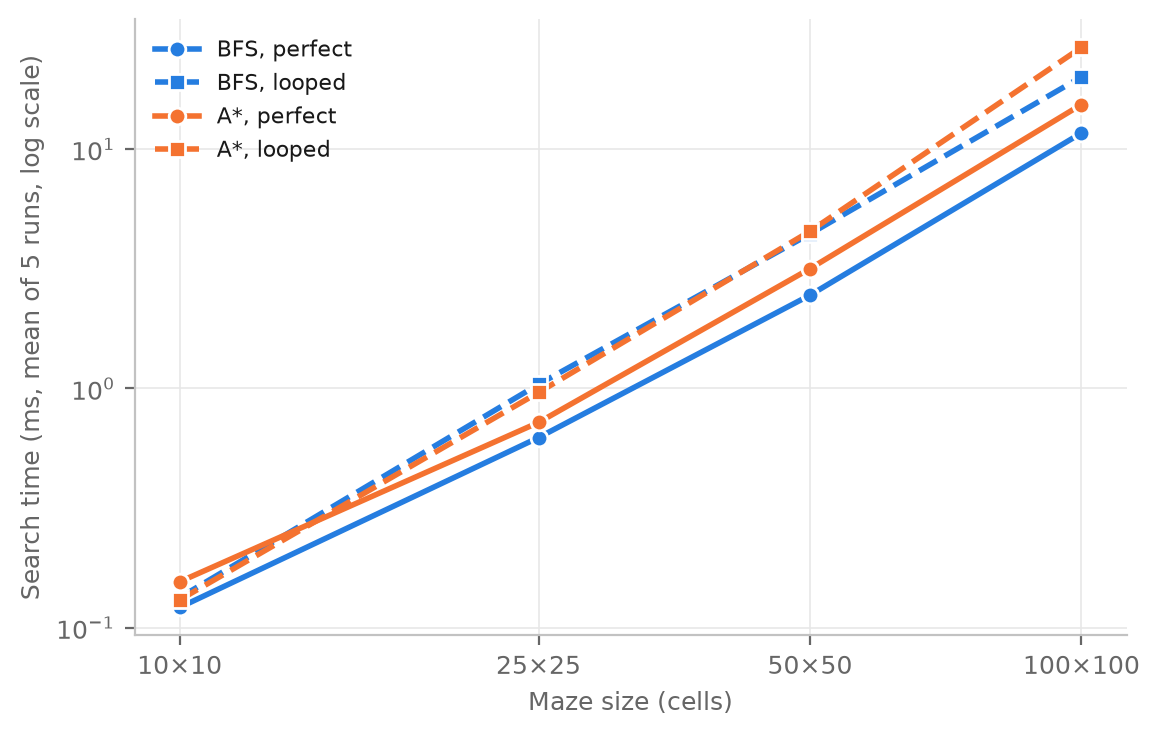
\includegraphics[width=\columnwidth]{figures/runtime_vs_size.png}
\caption{Search time against maze size (final seeds 10000 to 10049, 50 mazes per point; each maze timed as the mean of five runs after one warm-up; both axes logarithmic). Times depend on the implementation and machine (Appendix A).}
\label{fig:runtime}
\end{figure}

Memory, measured as the peak frontier size, is small for both algorithms because maze corridors are narrow: at 100$\times$100 the mean peak was 13 records for BFS and 13 for A* on perfect mazes, and 106 and 243 on looped mazes (Fig.~\ref{fig:frontier} in Appendix B). The A* frontier is larger because it keeps postponed branches with high f on the heap, where BFS discards each level as it goes. The dominant memory cost for both is the reached table, which is proportional to the number of squares.


\subsection{Limitations and what this experiment can and cannot establish}

\textbf{What the evidence supports.}

\begin{itemize}
  \item On mazes from this generator, with corner-to-corner queries, A* with Manhattan distance never returned a worse path than BFS and almost never expanded more nodes, across sizes from 10$\times$10 to 100$\times$100.
  \item Its advantage is small on perfect mazes and substantial on looped mazes, and it is predicted well by the informedness h(start)/C*.
  \item The advantage also depends on tie-breaking once many nodes share f = C*, and it shrinks when costs make the heuristic a looser bound.
\end{itemize}

\textbf{What it does not establish.}

\begin{itemize}
  \item \textbf{Other maze generators.} We used only the randomized depth-first generator, which makes long winding corridors. Prim's or Kruskal's algorithms make shorter dead ends and more direct solution paths, so the perfect-maze numbers could look different. The informedness analysis suggests how, but we did not test it.
  \item \textbf{Other queries.} Start and goal are always in opposite corners, the longest straight-line distance in the grid. Random start and goal pairs would include short queries where the heuristic matters less.
  \item \textbf{Other heuristics and move sets.} Only four-way moves and Manhattan distance were studied. We do not claim anything about eight-way movement or about stronger heuristics.
  \item \textbf{Runtime in general.} Timings come from one pure-Python implementation on one machine. A compiled implementation or a different priority queue would change the break-even point.
  \item \textbf{Causes.} Informedness is correlated with savings; we varied it only through the loop rate (and mud), so we cannot separate it from other things that change when walls are removed, such as the number of shortest paths. The explanation for the size trend in looped mazes (Section IV-B) is a hypothesis.
  \item \textbf{Scale.} The largest maze has about 40,000 squares. Trends beyond 100$\times$100 are extrapolation.
\end{itemize}

\section{Conclusions and Future Work}

\textbf{RQ1.} A* with Manhattan distance always returned a shortest path, and all 9,350 runs passed independent verification. On perfect mazes it expanded only 6.3\% (50$\times$50) and 3.7\% (100$\times$100) fewer nodes than BFS, so the 30\% target was not met. On looped mazes it saved 38.1\% and 24.4\%; the target was met at 50$\times$50 and not met at 100$\times$100. \textbf{RQ2.} The heuristic stops helping when it is uninformed, which we measured as h(start)/C*: below 0.4, A* reached 30\% savings on 13 of 248 mazes, and above 0.9 on 686 of 686. It also stops helping, in a different way, when it is exact but many nodes tie at f = C*: on open grids FIFO tie-breaking saved nothing while larger-g tie-breaking saved up to 99\%. \textbf{RQ3.} With mud, UCS and A* always found the same optimal cost, A* expanded 3.1\% to 19.6\% fewer nodes at the default mud rate depending on size, and BFS paths cost 3.8\% to 5.9\% more than the optimum on average.


\textbf{Lessons.}

\begin{itemize}
  \item The value of a heuristic is a property of the heuristic \emph{in an environment}. The same admissible, consistent heuristic was nearly useless in one family of mazes and excellent in another.
  \item Fair baselines and exact counting rules matter. Our own plan first used a counting rule that would have been off by one from the lecture example; reproducing a known result caught it before any experiment ran.
  \item Details that textbooks treat as footnotes, such as tie-breaking and the timing of the goal test, can decide the outcome: one line of tie-breaking moved savings from 0\% to over 90\% on open grids.
  \item Expansions and runtime are different measures. A* needed about 35\% fewer expansions just to match the running time of BFS in our implementation.
  \item Setting a success criterion in advance and reporting a miss was more informative than a criterion we would certainly have met.
\end{itemize}

\textbf{Future work.}

\begin{itemize}
  \item \textbf{Other maze textures:} repeat the study with Prim's and Kruskal's generators to test whether informedness predicts savings across generators, not just across loop rates.
  \item \textbf{Better heuristics for tree-like mazes:} dead-end filling as preprocessing, or a learned heuristic in the spirit of Neural A*~\cite{ref10}, evaluated on held-out seeds exactly as here.
  \item \textbf{Symmetry breaking on open grids:} Jump Point Search~\cite{ref8}, and eight-way movement with the Chebyshev (or octile) distance that it requires for admissibility~\cite{ref13}.
  \item \textbf{Uncertain moves:} if moves can slip, the maze becomes a Markov decision process, the Grid World of the course~\cite{ref13}, and value iteration replaces search.
  \item \textbf{Memory-bounded and bidirectional search:} IDA* and bidirectional BFS are natural competitors when the reached table, rather than the frontier, is the limit.
  \item \textbf{Changing mazes:} open or close walls during the search and compare repeated A* with incremental replanning such as D* Lite~\cite{ref17}.
\end{itemize}

\section{Individual Contribution and Professionalism}
\begin{table*}[!t]
\centering
\footnotesize
\setlength{\tabw}{\dimexpr \textwidth-6\tabcolsep\relax}
\caption{Responsibility of each member for the code components and the report sections.}
\label{tab:contrib}
\begin{tabular}{>{\raggedright\arraybackslash}p{\dimexpr 0.1697\tabw\relax}>{\raggedright\arraybackslash}p{\dimexpr 0.4121\tabw\relax}>{\raggedright\arraybackslash}p{\dimexpr 0.4182\tabw\relax}}
\toprule
\textbf{Member} & \textbf{Code} & \textbf{Report} \\
\midrule
Aaliyan Muhammad & Search loop, BFS, UCS, A*, heuristics, tie rules, greedy; hand-traced known-answer tests and search property tests & Search methods, heuristic proofs, side tests (tie rule, goal test and weighted A* ablations); limitations \\
Austin Brown & Perfect and looped maze generators, seed sets; generator tests and maze fingerprints & Problem setup, maze generation, loop rate sweep; heuristic informedness analysis \\
Aryan Farhang & Built the mud maze generator (looped mazes only) and the test that matches the Week 3 lecture numbers; ran the experiments and checked the results; wrote the README & Background and related work, mud maze results, reference list \\
Ki il Eum & Path checker, experiment runner, timing, statistics, one-command rerun; configuration files, code freeze and decision log & Testing and evaluation methods, main results table, answer to the 30\% target, reproducibility appendix; runtime and memory results \\
Yicheng Luo & All figures and charts, failure case figure, animated GIF; extra figures for Appendix B & Report lead: abstract, introduction, conclusion, title question write-up, contribution table, final self-grading and proofread; failure case discussion and future work \\
\bottomrule
\end{tabular}
\end{table*}

The split follows the roles in the proposal with two changes. Uniform Cost Search moved from Aryan Farhang to Aaliyan Muhammad, because all four algorithms share one search loop and are easier to keep consistent under one owner. Reproducing the Week 3 lecture example moved from Ki il Eum's test work to Aryan Farhang, because it exercises the weighted costs that the mud mazes depend on.


The results were not taken on trust. They were checked by means that do not depend on any one piece of code being right:

\begin{itemize}
  \item the automated test suite (1056 passed), including hand-traced expansion orders on small grids;
  \item exact reproduction of the costs and expansion counts of the Week 3 lecture example (Table~\ref{tab:lecture});
  \item an independent verifier, sharing no code with the search, on every one of the 9,350 final runs;
  \item a code freeze (git tag) before the final seeds were generated, with every design choice logged beforehand;
  \item a second full run of the final configuration, which reproduced the results file exactly (all 9,350 rows) except for the timing columns (Appendix A).
\end{itemize}

Each member also reviewed the code for their own part. Aaliyan Muhammad read the search loop and the heuristic code, traced the small known-answer grids by hand and compared them with the tests, and checked the admissibility and consistency proofs. Austin Brown read the generator and inspected rendered perfect, looped and weighted mazes for their expected structure. Aryan Farhang reran the test suite and the quick run, compared the lecture-example numbers with the Week 3 slides, and checked each reference against its source. Ki il Eum read the verifier and the experiment runner and confirmed with the comparison script that the second full run matched the results file. Yicheng Luo checked every figure against the tables it summarises, and edited and proofread the report.


\textbf{Professionalism and integrity.} All data in this report are synthetic and were generated by the submitted code from the listed seeds; no external data set was used. Every number, table and figure is produced by a script from the final results file, and the results file, metadata and seeds are submitted with the code. The success criterion was fixed in the proposal and is reported as stated, including where it was not met. The work is tracked in a public git repository, \texttt{https:/\allowbreak{}/\allowbreak{}github.com/\allowbreak{}AryanFP/\allowbreak{}maze-runner}, submitted with the code: each member committed their own part and merged it through a pull request, the tag \texttt{v1.0-final-run} records the code freeze, and every design choice that could change a number is logged with its reason in \texttt{DECISIONS.md} before the final run.

\appendices
\begin{table*}[!t]
\centering
\footnotesize
\setlength{\tabw}{\dimexpr \textwidth-18\tabcolsep\relax}
\caption{Additional metrics for the main experiment (final seeds 10000 to 10049, 50 mazes per row; means over mazes). The Wilcoxon signed-rank test is one-sided (A* expands fewer nodes than BFS).}
\label{tab:extra}
\begin{tabular}{>{\raggedright\arraybackslash}p{\dimexpr 0.1012\tabw\relax}>{\raggedright\arraybackslash}p{\dimexpr 0.1012\tabw\relax}>{\raggedleft\arraybackslash}p{\dimexpr 0.1131\tabw\relax}>{\raggedleft\arraybackslash}p{\dimexpr 0.1131\tabw\relax}>{\raggedleft\arraybackslash}p{\dimexpr 0.1131\tabw\relax}>{\raggedleft\arraybackslash}p{\dimexpr 0.1131\tabw\relax}>{\raggedleft\arraybackslash}p{\dimexpr 0.1190\tabw\relax}>{\raggedleft\arraybackslash}p{\dimexpr 0.1190\tabw\relax}>{\raggedleft\arraybackslash}p{\dimexpr 0.1071\tabw\relax}}
\toprule
\textbf{Maze type} & \textbf{Size} & \textbf{BFS generated} & \textbf{A* generated} & \textbf{BFS peak frontier} & \textbf{A* peak frontier} & \textbf{BFS median time (ms)} & \textbf{A* median time (ms)} & \textbf{Wilcoxon p} \\
\midrule
Perfect & 10$\times$10 & 119 & 107 & 3 & 3 & 0.12 & 0.15 & 1.2e-09 \\
Perfect & 25$\times$25 & 678 & 603 & 6 & 5 & 0.60 & 0.71 & 5.5e-10 \\
Perfect & 50$\times$50 & 2,614 & 2,460 & 8 & 8 & 2.40 & 3.05 & 3.8e-10 \\
Perfect & 100$\times$100 & 11,728 & 11,299 & 13 & 13 & 11.46 & 15.20 & 3.8e-10 \\
Looped & 10$\times$10 & 151 & 93 & 8 & 8 & 0.13 & 0.13 & 3.8e-10 \\
Looped & 25$\times$25 & 1,212 & 722 & 25 & 34 & 1.01 & 0.93 & 8.9e-16 \\
Looped & 50$\times$50 & 5,152 & 3,379 & 52 & 93 & 4.30 & 4.43 & 3.8e-10 \\
Looped & 100$\times$100 & 20,928 & 16,583 & 106 & 243 & 19.84 & 26.48 & 8.9e-16 \\
\bottomrule
\end{tabular}
\end{table*}

\section{Reproducibility}
\begin{table}[!t]
\centering
\footnotesize
\setlength{\tabw}{\dimexpr \columnwidth-4\tabcolsep\relax}
\caption{Environment and settings of the final run (from results/final/metadata.json).}
\label{tab:env}
\begin{tabular}{>{\raggedright\arraybackslash}p{\dimexpr 0.2182\tabw\relax}>{\raggedright\arraybackslash}p{\dimexpr 0.7818\tabw\relax}}
\toprule
\textbf{Item} & \textbf{Value} \\
\midrule
Repository & https://github.com/AryanFP/maze-runner \\
Code version & git tag v1.0-final-run (commit a65e8faf4c9c). The run recorded one modified tracked file, report/docx\_helpers.py (report formatting only). Nothing under src/, tests/ or config/ differed from the tag. \\
Final run started (UTC) & 2026-11-25T03:21:46+00:00 \\
Python & 3.13.6 (CPython). The proposal named 3.12; nothing depends on the difference. \\
Packages & numpy 2.5.5, pandas 3.1.1, matplotlib 3.11.2, scipy 1.18.1, pytest 9.2.0, pillow 13.0.0, python-docx 1.2.0 \\
Operating system & Windows-11-10.0.26200-SP0 \\
Processor & AMD64 Family 25 Model 33 Stepping 2, AuthenticAMD (12 logical cores) \\
Data provenance & All mazes are synthetic, generated by src/maze\_runner/generator.py from the seeds in Table~\ref{tab:seeds}. No external data. \\
Fixed settings & Loop rate p = 0.1; mud rate m = 0.2; mud cost 5; neighbour order Up, Right, Down, Left; A* tie rule larger-g; BFS goal test at generation; start (1, 1), goal (2n$-$1, 2n$-$1). \\
Counting rule & Expanded = removed from the frontier, not stale, not the goal, successors generated. \\
Test summary & 1056 passed in 4.06s \\
Verification & 9,350 of 9,350 runs legal; 7,550 of 7,550 optimal where optimality is guaranteed. \\
Bootstrap & Percentile method, 10,000 resamples of mazes, random seed 3346. \\
\bottomrule
\end{tabular}
\end{table}

\textbf{Commands} (from the repository root, after \texttt{pip install -r requirements.txt} and \texttt{pip install -e .}):

{\scriptsize\begin{verbatim}
python -m pytest -q         # run all tests
python run_all.py --quick   # small check run (about a minute)
python run_all.py           # tests, experiments, figures, report
python -m maze_runner.experiment config/final.json \
       --out results/repro_check
\end{verbatim}}

The repository contains the final results file (results/final/runs.csv, one row per maze and configuration, with the maze fingerprint, all counters, the verification columns and the timings), the metadata file, the tables behind every table in this report (results/final/tables), all figures, the development results, the decisions log, and an animated comparison of BFS and A* (results/final/figures/bfs\_vs\_astar.gif). We reran the final configuration into a separate folder and compared the two files with tools/compare\_runs.py: they are identical except for the three timing columns. Known limitations are listed in Section IV-H, and the division of labour in Section VI.


\section{Additional tables and figures}

Table~\ref{tab:extra} and Fig.~\ref{fig:frontier} give the remaining metrics of the main experiment: nodes generated, peak frontier size, median search time and the paired significance test.

\begin{figure}[!t]
\centering
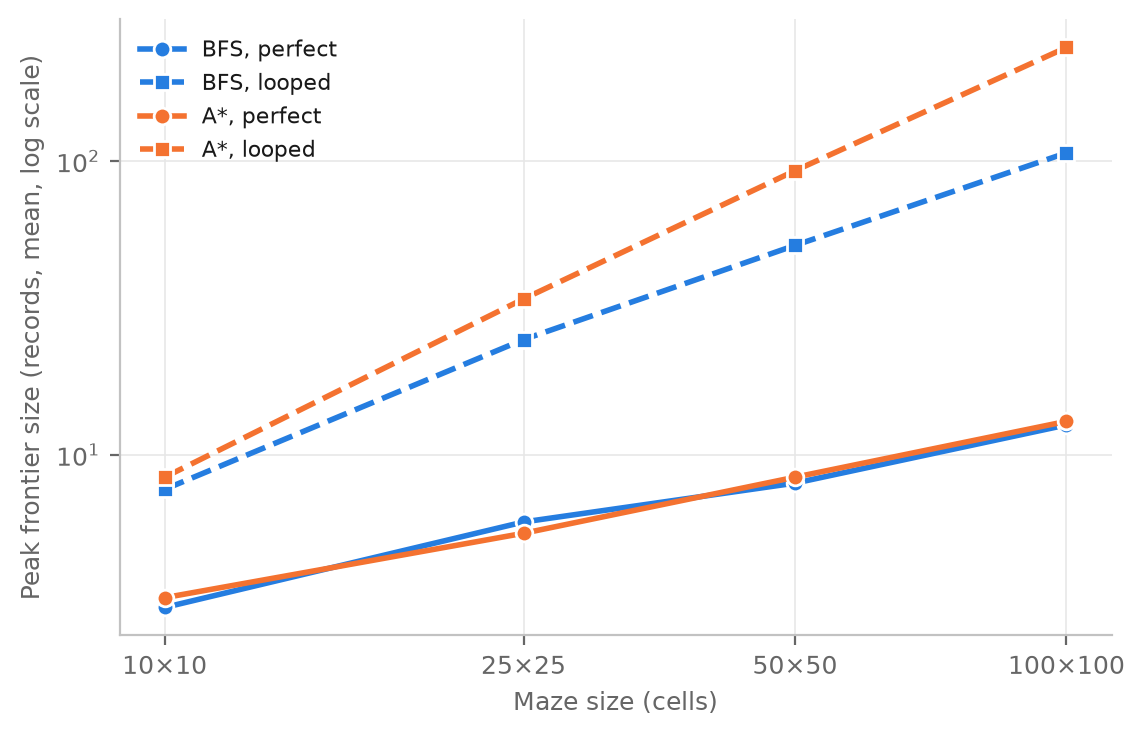
\includegraphics[width=\columnwidth]{figures/peak_frontier_vs_size.png}
\caption{Peak frontier size against maze size (final seeds 10000 to 10049, 50 mazes per point; both axes logarithmic). For A* the count includes stale heap records.}
\label{fig:frontier}
\end{figure}

\begin{thebibliography}{00}
\bibitem{ref4} S. Russell and P. Norvig, \emph{Artificial Intelligence: A Modern Approach}, 4th ed. Pearson, 2021.
\bibitem{ref1} P. E. Hart, N. J. Nilsson and B. Raphael, ``A formal basis for the heuristic determination of minimum cost paths,'' \emph{IEEE Transactions on Systems Science and Cybernetics}, vol. 4, no. 2, pp. 100--107, 1968.
\bibitem{ref13} B. Davis, \emph{CS3346A Introduction to Artificial Intelligence}, lecture slides: Lecture 2 (Augmenting intelligence and searching state spaces), Week 3 (Heuristics and graph search), Week 6 (Markov decision processes), Week 10 (Learning and evaluation). Western University, Fall 2026.
\bibitem{ref3} E. F. Moore, ``The shortest path through a maze,'' in \emph{Proceedings of the International Symposium on the Theory of Switching}, Part II, Harvard University Press, 1959, pp. 285--292.
\bibitem{ref2} E. W. Dijkstra, ``A note on two problems in connexion with graphs,'' \emph{Numerische Mathematik}, vol. 1, pp. 269--271, 1959.
\bibitem{ref5} J. Pearl, \emph{Heuristics: Intelligent Search Strategies for Computer Problem Solving}. Addison-Wesley, 1984.
\bibitem{ref6} R. Dechter and J. Pearl, ``Generalized best-first search strategies and the optimality of A*,'' \emph{Journal of the ACM}, vol. 32, no. 3, pp. 505--536, 1985.
\bibitem{ref9} J. Buck, \emph{Mazes for Programmers: Code Your Own Twisty Little Passages}. Pragmatic Bookshelf, 2015.
\bibitem{ref7} N. R. Sturtevant, ``Benchmarks for grid-based pathfinding,'' \emph{IEEE Transactions on Computational Intelligence and AI in Games}, vol. 4, no. 2, pp. 144--148, 2012.
\bibitem{ref8} D. Harabor and A. Grastien, ``Online graph pruning for pathfinding on grid maps,'' in \emph{Proceedings of the AAAI Conference on Artificial Intelligence}, 2011, pp. 1114--1119.
\bibitem{ref12} I. Pohl, ``Heuristic search viewed as path finding in a graph,'' \emph{Artificial Intelligence}, vol. 1, no. 3--4, pp. 193--204, 1970.
\bibitem{ref10} R. Yonetani, T. Taniai, M. Barekatain, M. Nishimura and A. Kanezaki, ``Path planning using Neural A* search,'' in \emph{Proceedings of the 38th International Conference on Machine Learning (ICML)}, PMLR 139, 2021, pp. 12029--12039.
\bibitem{ref11} L. Lehnert, S. Sukhbaatar, D. Su, Q. Zheng, P. McVay, M. Rabbat and Y. Tian, ``Beyond A*: Better planning with transformers via search dynamics bootstrapping,'' arXiv preprint arXiv:2402.14083, 2024.
\bibitem{ref16} R. E. Korf, M. Reid and S. Edelkamp, ``Time complexity of iterative-deepening-A*,'' \emph{Artificial Intelligence}, vol. 129, no. 1--2, pp. 199--218, 2001.
\bibitem{ref14} M. Helmert and G. R\"oger, ``How good is almost perfect?,'' in \emph{Proceedings of the Twenty-Third AAAI Conference on Artificial Intelligence (AAAI-08)}, 2008, pp. 944--949.
\bibitem{ref15} M. Asai and A. Fukunaga, ``Tiebreaking strategies for A* search: How to explore the final frontier,'' in \emph{Proceedings of the Thirtieth AAAI Conference on Artificial Intelligence (AAAI-16)}, 2016, pp. 673--679.
\bibitem{ref17} S. Koenig and M. Likhachev, ``D* Lite,'' in \emph{Proceedings of the Eighteenth National Conference on Artificial Intelligence (AAAI-02)}, 2002, pp. 476--483.
\end{thebibliography}
\end{document}
